\documentclass[12pt]{report}

\providecommand{\E}[1]{\ensuremath{\times 10^{#1}}}
\usepackage{graphicx}% Include figure files
\usepackage{amsmath}
\usepackage{amsfonts}
\usepackage{amssymb}

\usepackage{natbib}
%\bibliographystyle{ieeetr}
\bibliographystyle{agufull08}
\setcitestyle{authoryear, square}

\usepackage{cleveref}
%\usepackage{caption}
\usepackage{subcaption}





% Vectors in bold font instead of line over
\renewcommand{\vec}[1]{\mathbf{#1}}
% Math-mode vector alternative (greek symbols)
\newcommand{\mvec}[1]{\boldsymbol{#1}}

% units in math mode
\newcommand{\unit}[1]{\quad[\mathrm{#1}]}

% Big fractions
\newcommand{\bigfrac}[2]{\ensuremath{\frac{\displaystyle #1}{\displaystyle #2}}}


% Exponential:
\renewcommand{\exp}[1]{e^{#1}}
\usepackage{suthesis-2e}
    \specialthesis

\dept{Electrical Engineering}


    \begin{document}
    \title{Global and Seasonal Effects of\\
            Lightning-Induced Electron Precipitation}
    \author{Austin Patrick Sousa}
    \principaladviser{Prof. Sigrid Close}
    \firstreader{Prof. Robert Marshall, University of Colorado Boulder}
    \secondreader{Prof. Antony Fraser-Smith} 
    \beforepreface
    \prefacesection{Preface}
        This thesis tells you all you need to know about...
    \prefacesection{Acknowledgments}
        This dissertation represents the culmination of my nearly seven years at Stanford, and I've been thinking about writing this section for the last three. And yet, sitting here at my desk at the University of Colorado, I find myself at a lack for words.

Going into a Ph.D program, you tend to think of a dissertation as a final, be-all, end-all answer, a pinnacle of unrelenting, focused, thoughtful research, culminating in The Great Answer to your questions. Now, at the end of my program, however, this dissertation feels oddly anticlimactic. My path to this point was by no means direct: graduate research is by nature a meander, a random walk trajectory through courses and projects and countless research papers. There's no straight line to the finish - but there is, with enough guidance, a drift. 

By no means would I say I've arrived at the fabled ``answer''. I don't feel a sense of enlightenment. My work here has left me with an ever-expanding set of questions, model improvements, approximations and assumptions in need of scrutiny. But in a sense that is the destination for the countless hopeful academics who have embarked on a Ph.D. At the end, there are only more questions.

My particular path through Stanford was not direct at all. I entered as a first year student in the VLF group, which focused on low-frequency radio waves in the magnetosphere. The VLF group was built on over 50 years of geophysics and radioscience research at Stanford, and consisted of a thriving collection of a half-dozen research staff and nearly twenty graduate students, under the direction of Dr. Umran Inan. I knew early on that the VLF group had reached the end of its lifespan going into it, but had been assured that things would continue smoothly, that there would be people to work with, and that I would be one of a handful of final students to carry the VLF banner.

Within my first couple years, I worked on several interesting and unique research opportunities -- beginning first with hardware design for a CubeSat (see chapter \ref{chapter:vpm}),

VLF waves traverse great distances, and research on these waves follows accordingly. The VLF group prided itself on maintaining a global network of student-maintained radio receivers, from Alaska to Antarctica. Less than two years in as a student, I found myself, along with fellow student Chris Young, dragging four heavy Pelican cases through the rush-hour crush of a train station in Kagoshima, Japan, as part of a ten-day stint installing three such receivers in Sapporo, Kagoshima, and Mt. Fuji. Similarly, I had been entrusted, along with a handful of other students, with designing a CubeSat -- which would go to space! -- which at the time felt both incredible and overwhelming. The excitement within the group was palpable, fueled by a driven professor and supported by the well-trained machinery of the senior research staff.

Unfortunately, things were somewhat built to spill, and as the quarters progressed steadily on, our ranks began to dwindle. Other groups brought in new students and new projects; but I was the last one in the door. The excitement dwindled; the research meetings grew smaller and smaller. Labs were shut down, equipment surplussed, and the open doors of professors remained frequently shut. 

As the group continued to shrink, my research advisor, Dr. Sigrid Close, graciously took me into her lab in the Aerospace Engineering department, along with VLF research scientists Dr. Robert Marshall and Dr. Ivan Linscott. Switching to the AA department was a fantastic opportunity to escape the loneliness and gloom of the Packard basement lab. Courses and research continued on, now in an active research group (and with daylight windows!). Not soon thereafter, however, Dr. Robert Marshall secured a coveted faculty position at CU Boulder. I found myself working on a project unrelated to my fellow students, and again lacked an in person mentor.

The fourth year was the hardest. By four years in, you've likely taken all the classes you need to, and hopefully have a start on a dissertation topic. But by four years, you're too far in to quit, and yet the end is nowhere in sight. Furthermore, with no remaining classes to count, you're truly cut free -- and without steady guidance, there's no obvious way forward.

-----------

There are countless people who, without their invaluable guidance, I would not be writing this section today. First and foremost, to my mentor, Dr. Robert Marshall, who has been perhaps the one constant thread throughout my seven years, first as a faculty mentor on the VPM project, then as a co-advisor in the AA department, and now as my PI at the University of Colorado. Bob, you're an inspiration.

To my advisor, Dr. Sigrid Close, who took me in despite having an already overwhelming cadre of students. I've always appreciated our conversations, and that you'd let them meander to topics across the board. As much as Bob would hone ideas in, Dr. Close would let brainstorming sessions run rampant.

To Dr. Antony Fraser-Smith, who as graciously served as my third committee member, especially while recovering from a heart surgery. Tony has been a part of the radioscience group at Stanford since the 1970s, and is a wellspring of interesting stories, entertaining anecdotes, and exudes the good-natured, jovial personality that makes geoscience a compelling world to work in. Furthermore, Dr. Fraser-Smith was responsible for putting together the Villard Fellowship for Students in Radioscience, in memory of the late Dr. Oswald Villard, which supported my first year of research, and was the deciding factor in my attending Stanford. 

To the researchers and engineers who kept the VLF group running: Dr. Ivan Linscott, Dr. Dave Lauben, Dr. Morris Cohen, who made themselves available for any and every question I had, no matter how trivial. A special thank you to Dr. Maria Spasojevic, who took the time to personally call me when I was applying to grad school.
 
To Jeff Chang, who singlehandedly ran every technical aspect of the VLF group, from the compute cluster to PCB layout to metal manufacturing.
 
To Professor Emiko Yasumoto in the Japanese language department, who showed special concern for my well-being during a particularly rough time. \begin{CJK}{UTF8}{min}??????????\end{CJK} \\

To my friends, colleagues, and lunch buddies from the VLF and SESS groups: Chris Young, with whom I've shared adventures across Japan; David Freese, for dragging me 5000 feet up Half Dome in the middle of the night; Patrick Blaes, who taught me everything I know about everything (no joke). To Rasoul Kabirzadeh, who started the same quarter as I did and went through many of the same struggles I encountered. To Nicholas, Sid, Anna, Lorenzo, and everyone in the SESS group who welcomed me in halfway through my program: Thank you all.

I owe a truly incalculable debt of gratitude to my community outside of campus, who without their constant companionship I most surely would have turned tail and returned to Seattle in 2012. To Ted Phares and Tristan Hudson, for 2am snacks and 2pm breakfast. To Damien Heiser and Wayne Tsai, for bringing me to Burning Man --Twice!\footnote{so far}. To Galen, Abe, JDT, Mike, Phil, Dan, Ricky, Hukka, Max, and everyone else: more than the classes, more than the research: you guys made me the person I am today, and I would not be here without you. Thank you.

To my former bosses and colleagues in the music industry, from my life before college, Bob Lang and Stuart Hallerman, for inspiring me to study electronics in the first place.

To my partner of nearly 9 years, Ty Logan: Thanks for putting up with me.

Finally, to my high school history teacher, Mark Rippy: In my senior year, I had to write a history paper and I refused to do it. Mark gave me some brief, offhand advice that hit me at just the right moment: ``Nobody else will do it for you." It was a bombshell, and it changed my life. It sounds silly, but those words became a mantra that got me through high school, an associate's degree, five years in the music industry, two bachelors degrees, a Master's degree, and now, a Stanford doctorate. Thank you.


    \afterpreface
 
    \chapter{Introduction}
    	\section{The Space Environment}
\section{Motivation}
\section{Previous Work}
\section{Thesis Organization}


    \chapter[Physics and Methods]{Background Physics and Description of Methods}
    	\section{Overview of Plasma Physics}
A \emph{plasma} is a quasi-neutral gas of ions, electrons, and neutral particles, which exhibit collective behavior. Plasmas can behave in similar ways to a conventional fluid -- they can flow, they can be compressible, they can be turbulent, and so on -- however the addition of charged particles facilitates many behaviors unique to a plasma. Charged particles can interact with each other not just through ballistic collisions, but at a distance through electromagnetic forces. The bulk motion of a plasma can be manipulated through electric and magnetic fields; conversely a plasma can have a substantial effect on the propagation of radio waves passing through it. 

A plasma can be analyzed in several different domains: Single particle motion; fluid approximations; and full kinematic solutions. In this work we treat the motions of electrons in the single particle domain, which is a natural choice for the sparse densities and small gyroradii of radiation belt electrons. To understand the behavior of radio waves propagating through a plasma, we treat the background as a smooth dielectric medium. 

\subsection{Single Particle Motion}
The high energies and sparse densities of the radiation belts lend themselves very well to a single-particle approximation. Many of the basic behaviors and quantities in plasma physics can be understood through studying the motion of a single particle.

The fundamental equation of motion for a charged particle in an electromagnetic field is given by the Lorentz force:
\begin{equation}
\vec{F} = \frac{d\vec{p}}{d\emph{t}} = q(\vec{E} + \vec{v}\times\vec{B})
\label{eqn:lorentz_force}
\end{equation}
Where $q$ represents the particle's charge, $\vec{E}$ and $\vec{B}$ represent the electric and magnetic fields, and $\vec{v}$ the particle's velocity, shown here in a non-relativistic frame.

Electric fields simply apply a force in the direction of the field. However, note that a cross product is perpendicular to both terms -- therefore any forces induced by the magnetic field will be perpendicular to the particle's velocity. The magnetic field is a \emph{conservative} force, in that a stationary magnetic field cannot directly impart energy into a particle, but can alter a particle's trajectory. The particle will therefore have a net drift in the direction of the electric field, while exhibiting a helical motion around the magnetic field.

We can then split the velocity vector into two quantities -- $v_\parallel$ parallel to the magnetic field, and $v_\perp$ perpendicular to the magnetic field.

Two characteristic values arise from this motion: the radius of the particle's rotation around the magnetic field, known as the \emph{gyroradius} or the \emph{Larmor radius}:
\begin{equation}
r_l = \frac{m v_\perp}{qB}
\end{equation}

And the rotation frequency, known as the \emph{gyrofrequency} or \emph{cyclotron frequency}:
\begin{equation}
\omega_c = \frac{v_\perp}{r_l} = \frac{q B}{m} \unit{rad/sec}
\end{equation}

By integrating the particle's momentum over a single gyrorotation, we arrive at a third fundamental quantity known as the magnetic moment, or the \emph{first adiabatic invariant}:
\begin{equation}
\mu = \frac{m v_\perp^2}{2B}
\label{eqn:mu}
\end{equation}

In situations where the magnetic field varies slowly (e.g., on spatial scales much greater than the gyroradius), then $\mu$ remains a constant of motion.

A final parameter to describe a particle's motion is it's \emph{pitch angle}, the angle between the velocities perpendicular and parallel to the magnetic field:
\begin{equation}
\alpha = \mathrm{tan}^{-1}\bigg(\frac{v_\perp}{v_\parallel}\bigg)
\end{equation}

The first adiabatic invariant describes an implicit relationship between the magnetic field strength and a particle's pitch angle at a given point. 
Combining the first adiabatic invariant with conservation of kinetic energy, we can deduce an expression for magnetic trapping -- that is, the magnetic field strength in which a particle exhibiting helical motion along a magnetic field line will turn around at. 
\begin{eqnarray}
& E &= \frac{1}{2}mv^2 \\
& &= \frac{1}{2}m(v_\parallel^2 + v_\perp^2) \\
 & &= \frac{1}{2}mv^2(\mathrm{cos}^2\alpha + \mathrm{sin}^2\alpha)
\end{eqnarray}

At a reflection point, the particle's kinetic energy will be entirely in the perpendicular mode:
\begin{eqnarray}
\frac{v_{\perp0}^2}{B_0} = \frac{v_{\perp1}^2}{B_1} \\
\frac{v^2\mathrm{sin}^2(\alpha)}{B_0} = \frac{v^2}{B_1} \\
\mathrm{sin}^2(\alpha)=\frac{B_0}{B_1} 
\end{eqnarray}

Therefore, a charged particle in a magnetic field will be constrained to rotate around a field line, and bounce back and forth, reflecting where the magnetic field strength increases. A key takeaway is that the reflection point is independent of energy, and depends only on the ratio of magnetic field strengths and the particle's initial pitch angle. An example of this behavior is shown in figure \ref{fig:bottle}.
\begin{figure}[ht]
\begin{center}
\includegraphics{figures/bottle.pdf}
\caption{An example of a ``magnetic bottle" particle trap. The top plot shows the trajectory of an electron with an initial pitch angle $\alpha_0=20^\circ$. The bottom plot shows the magnetic field ratio $B_0/B_1$, with the particle's reflection points shown as vertical lines. }
\label{fig:bottle}
\end{center}
\end{figure}


\subsection{Waves in Plasmas}
Previously, we have described the motion of a charged particle under the influence of an electromagnetic field. the single-particle approximation provides enormous insight into the dynamics of a sparsely-populated plasma. Next, we must consider the inverse system -- how the charged particles in a plasma dictate the characteristic behaviors of an electromagnetic wave propagating through it.

An electromagnetic wave can accelerate a charged particle; conversely, an accelerating or decelerating particle induces its own electromagnetic field. It would seem, then, that the behavior of an electromagnetic field in a plasma is simply the summation of the contributions of each particle and some incident wave source. However, the complexity of this brute-force approach quickly becomes intractable for even a handful of particles. The universal approach taken then is to abstract the complicated interplay of waves and particles into a wave moving through a dielectric medium, described only by the various constituent densities, temperatures, and background field intensities within a given volume. 

As with any electromagnetic problem, we begin with Maxwell's equations -- shown here in their non-relativistic, differential form, in SI units:

\begin{eqnarray}
&\nabla \cdot \vec{E}& = \frac{\rho}{\epsilon_0} \label{eqn:maxwell1}\\
&\nabla \cdot \vec{B}& = 0 \label{eqn:maxwell2}\\
&\nabla \times \vec{E}& = -\frac{\partial \vec{B}}{\partial t} \label{eqn:maxwell3}\\
&\nabla \times \vec{B}& = \mu_0 \vec{J} + \frac{1}{c^2}\frac{\partial \vec{E}}{\partial t} \label{eqn:maxwell4}
\end{eqnarray}

$\vec{E}$ and $\vec{B}$ denote the electric and magnetic fields; $\mu_0$ and $\epsilon_0$ denote the magnetic permeability and electric permittivity of free space; and $c=\sqrt{\frac{1}{\mu_0\epsilon_0}}$ is the speed of light. The terms $\rho$ and $\vec{J}$ represent the local charge density and current density, both of which may be functions of position and time.

By taking the curl of equation \ref{eqn:maxwell3} and substituting in the time derivative of equation \ref{eqn:maxwell4}, and making use of the vector identity $\nabla \times \nabla \times \vec{E} = \nabla(\nabla \cdot \vec{E}) - \nabla^2\vec{E}$, we have:

\begin{equation}
\nabla^2\vec{E} - \frac{\nabla\rho}{\epsilon_0} = \mu_0 \frac{\partial \vec{J}}{\partial t} + \frac{1}{c^2}\frac{\partial^2\vec{E}}{\partial t^2}
\label{eqn:dielectric_tensor_derivation_1}
\end{equation}

In the absence of charges or currents ($\rho=0$, $\partial\vec{J}/\partial t=0$), the equation reduces to the free-space wave equation:
\begin{equation}
\nabla^2\vec{E} = \frac{1}{c^2}\frac{\partial^2\vec{E}}{\partial t^2}
\end{equation}

Next, we linearize the system and search for harmonic perturbations of the form:
\begin{eqnarray}
\vec{E(\vec{r},t)} = \vec{E_1}e^{{i (\omega t - \vec{k}\cdot \vec{r}})} \label{eqn:linear1}\\ 
\vec{B(\vec{r},t)} = \vec{B_0} + \vec{B_1}e^{{i (\omega t - \vec{k}\cdot \vec{r}})} \label{eqn:linear2}\\
\vec{J(\vec{r},t)} = \vec{J_1}e^{{i (\omega t - \vec{k}\cdot \vec{r}})}\label{eqn:linear3} 
\end{eqnarray}

where $\omega$ is the wave angular frequency, $\vec{k}$ is the wave vector, or spatial frequency, and $\vec{r}$ is the spatial coordinate. Two fundamental parameters of an electromagnetic wave are the \emph{phase velocity}, $\omega/k$, and the \emph{group velocity}, $\partial\omega/\partial k$. The relation between the temporal and spatial frequencies is known as the \emph{dispersion relation}.

From here we follow the derivation and convention used by \cite{Stix1992} and \cite{Bittencourt2004}. In general, a plasma is comprised of several different species of constituent particles -- positively and negatively charged particles necessary to maintain a quasi-neutral plasma. While the dispersion relations of different species cannot be simply added, their effects can be summed to form the displacement current $\vec{J}$:
\begin{equation}
\vec{J} = \sum_s\vec{J_s} = \sum_s n_s q_s \vec{u_s}
\label{eqn:J}
\end{equation}
where $n$, $q$, and $\vec{u}$ represent the (number) density, charge, and velocity of a particular species $s$. 

We make the assumption that the plasma is \emph{cold} -- that is, that the velocities of each species $\vec{u_s}$ have a single value each. Were we to relax this assumption, each species density would have a distribution function in both position and momentum, $n=n(\vec{r},\vec{p})$; the total current would then be an integration over momentum for each species. For a treatment of a hot plasma, see the work by \cite{Sazhin1993}.

Next, we note that, in a cold plasma assumption, the Lorentz force (equation \ref{eqn:lorentz_force}) can be written for each species:
\begin{equation}
m_s\frac{d\vec{u_s}}{dt} = q_s\big(\vec{E} + \vec{u_s}\times\vec{B}\big) 
\label{eqn:lorentz_2}
\end{equation}
Combining equations \ref{eqn:linear1} -- \ref{eqn:linear3}, \ref{eqn:J}, and \ref{eqn:lorentz_2}, and assuming a coordinate system with the background magnetic field $\vec{B_0}$ aligned with the z-axis, we arrive at an expression for the \emph{cold-plasma dielectric tensor}:

\begin{equation}
\mvec{\epsilon}\cdot\vec{E}=\begin{pmatrix}
S & -iD & 0 \\
iD & S & 0 \\
0 & 0 & P \end{pmatrix}\begin{pmatrix}E_x \\ E_y \\ E_z\end{pmatrix}
\end{equation}

The various summations over each constituent species are incorporated into the so-called Stix parameters (\cite{Stix1992}):
\begin{eqnarray}
S =\frac{1}{2}(R + L) \qquad D = \frac{1}{2}(R - L)
\label{eqn:stix_params_1}
\end{eqnarray}
\begin{equation}
R = 1 - \sum_s\frac{\omega_{ps}^2}{\omega(\omega + \omega_{cs})}; \quad L = 1 - \sum_s\frac{\omega_{ps}^2}{\omega(\omega - \omega_{cs})}; \quad P = 1 - \sum_s\frac{\omega_{ps}^2}{\omega^2}
\label{eqn:stix_params_2}
\end{equation}

where $\omega_{ps} = n_sq_s^2/{\epsilon_0 m_s}$ and $\omega_{cs}=q_sB_0/m_s$ are the plasma and cyclotron frequencies for species $s$.

\subsubsection{Dispersion Relation}
With the dielectric tensor now determined, we can derive the relationship between $\omega$ and $\vec{k}$, known as the dispersion relation. Equation \ref{eqn:dielectric_tensor_derivation_1} can be written as:
\begin{equation}
\mvec{\eta}\times \mvec{\eta} \times \vec{E} +  \mvec{\epsilon}\cdot\vec{E} = 0
\end{equation}
where $\mvec{\eta} = \vec{k}c/\omega$ is the wave refractive index. Assuming a wave propagating with some angle $\theta$ between $\mvec{\eta}$ and the background magnetic field, we arrive at:
\begin{equation}
\begin{pmatrix}
S - \eta^2\cos^2\theta & -iD & \eta^2\cos{\theta}\sin{\theta} \\
iD & S - \eta^2 & 0 \\
\eta^2\cos{\theta}\sin{\theta} & 0 & P - \eta^2\sin^2{\theta} \end{pmatrix}\begin{pmatrix}E_x \\ E_y \\ E_z\end{pmatrix} = 0
\label{eqn:dispersion_relation_matrix}
\end{equation}

Taking the determinant of \ref{eqn:dispersion_relation_matrix} yields the \emph{cold-plasma dispersion relation}:

\begin{eqnarray}
&A\eta^4 - B\eta^2 + C &= 0 \label{eqn:disp_rln}  \\
&A& = S \sin^2\theta + P\cos^2\theta \\
&B& = RL\sin^2\theta + PS(1 + \cos^2\theta) \\
&C& = PRL
\end{eqnarray}

Equation \ref{eqn:disp_rln} is biquadratic -- we can solve for $\eta^2 = k^2c^2/\omega^2$ using the quadratic formula.

Finally, it is worth noting that when considering a single-species plasma (e.g., electrons only), equation \ref{eqn:disp_rln} reduces to the well-known \emph{Appleton-Hartree Equation} (\cite{Appleton1932}):


\begin{equation}
\eta^2 = 1 - \frac{\frac{\omega_{pe}^2}{\omega^2}}{1 - \frac{\omega_{ce}^2\sin^2\theta}{2(\omega^2 - \omega_{pe}^2)} \pm\big[\big(\frac{\omega_{ce}^2\sin^2\theta}{2(\omega^2 - \omega_{pe}^2)}\big)^2 + \frac{\omega_{ce}^2}{\omega^2}\cos^2\theta\big]^{1/2}}
\end{equation}

%For a simpler derivation of the Appleton-Hartree equation alone, see the classic, approachable text by \cite{Chen1983}.  %% (CHEN DOESN'T SEEM TO DO IT x.x) 

The dispersion relation in equation \ref{eqn:disp_rln} reveals a wealth of information about the characteristics of waves in plasmas. For various plasma densities and background magnetic field strength, we can infer which wave frequencies may propagate, if any, and which wave polarizations. Through the remainder of this work, we will be concerned with the \emph{Whistler} mode -- a right-hand, circularly-polarized (RHCP) wave. Within a typical magnetospheric plasma, the Whistler mode spans the VLF band, roughly between 30 Hz and 300 kHz.

Figure \ref{fig:whistler_mode_dispersion} shows a typical dispersion relation for a magnetospheric plasma (L $\approx$ 2) by plotting frequency vs wavenumber ($\eta = k c/\omega$). The Whistler mode is the lower branch of the RHCP mode.
\begin{figure*}[ht]
\begin{center}
\includegraphics{figures/omega-k_diagram_parallel}
\caption{An $\omega$-K diagram for the cold plasma dispersion relation, shown here for a wave propagating parallel to $\vec{B}$, in four-component plasma with $N_e \approx  6\E{8}\,e^-/m^3$, and $B\approx 4\,\mu T$. For higher frequencies the dispersion relation asymptotes to the free-space solution, with slope $c$. The Whistler mode is the right-hand, circularly-polarized mode which spans the majority of the frequency band. The shaded region marks the characteristic band in which the right-hand mode cannot propagate. At lower frequencies, the left-hand circular mode resonates with the various ion constituents,  known as the \emph{Ion Cyclotron} modes.}
\label{fig:whistler_mode_dispersion}
\end{center}
\end{figure*}

\section{Lightning Illumination Model}
%\subsection{Emission Spectrum}
A single lightning flash is a stochastic dielectric breakdown process. While a terrestrial lightning flash consists of several repeated strokes at varying incident angles, we adopt the simplified model used by \citealt{Lauben1998}, \citealt{Bortnik2005}, and subsequent workers.

The lightning flash is modeled as a single, vertical current pulse from a height $H_E$, with a time profile given by equation \ref{eqn:td_pulse}:
\begin{equation}
\label{eqn:td_pulse}
I(t)=I_0(e^{-a t} - e^{-b t})
\end{equation}

We relate the time-domain current profile to radiated power using the far-field approximation for an arbitrary source, given by \cite{Griffiths1999}, page 457:
\begin{equation}
\label{eqn:griffiths_power}
S(t) \approx \frac{1}{\mu_0}(\mathbf{E} \times \mathbf{B}) = \frac{\mu_0}{16\pi^2c}\left[\ddot{p}(t)\right]^2 \left(\frac{\sin^2\theta}{r^2}\right)\mathbf{\hat{r}}
\end{equation}

where $p(t)$ is the dipole moment given by $p=2 H_E \int_0^t{I(t)}dt$, r is the distance from the flash in meters, and $\theta$ is the angle to the flash. Taking the second derivative of the dipole moment (the first derivative of the current profile) gives us the far-field time-domain power equation:

\begin{equation}
\label{eqn:farfield_power_td}
S(t) = \frac{1}{Z_0}\left(\frac{\mu_0 H_E I_0}{2 \pi}\right)^2\left(\frac{\sin^2\theta}{r^2}\right) \left(a e^{-a t} - b e^{-b t}\right)^2  \mathbf{\hat{r}}
\end{equation}

where we have used the relation $Z_0 = \mu_0 c$. Equation \ref{eqn:farfield_power_td} has units of energy flux density, Watts per square meter ($J/m^2/$sec).

To determine the frequency spectrum of the radiated power, we take the Fourier transform of equation \ref{eqn:farfield_power_td}:

\begin{equation}
\label{eqn:farfield_power_fd}
S(\omega) = \frac{1}{Z_0}\left(\frac{\mu_0 H_E I_0}{2 \pi}\right)^2\left(\frac{\sin^2\theta}{r^2}\right) \frac{\omega^2(a-b)^2}{(\omega^2 + a^2)(\omega^2 + b^2)}  \mathbf{\hat{r}}
\end{equation}

which has units of energy flux per frequency -- J/m$^2$/Hz.

Throughout this work we assume a flash height $H_E$=5 km, and model parameters $a=5\E{3}\,\mathrm{sec}^{-1}$ and $b=1\E{5}\,\mathrm{sec}^{-1}$, resulting in a spectrum peaked at approximately 4kHz; any lightning flash can be parameterized solely by its peak current $I_0$ and its location on the surface of the Earth. Figure \ref{fig:lightning_spectrum} shows the current profile and associated spectrum.

\begin{figure*}
\begin{center}
\includegraphics{figures/Lightning_spectra.pdf}

\caption{Double-exponential current pulse model of a lightning stroke. The top panel shows the stroke current vs time; the middle panel shows the total energy flux, integrated over space, vs time; the bottom panel shows the energy flux in the frequency domain.}
\label{fig:lightning_spectrum}
\end{center}
\end{figure*}


\section{The Ionosphere}
The ionosphere, extending from $\approx$ 85 km to 1000 km, is the highly-variable transition region between the terrestrial neutral atmosphere and the sparse plasmas of the space environment. The relatively-sharp rise in electron density at the bottom of the ionosphere makes it highly-reflective within the VLF band, forming a waveguide between it and the conductive surface of the Earth. However, In studying LEP, we are primarily concerned with the fraction of energy which does not reflect, and instead propagates through the ionosphere and out into the plasmasphere.

\subsection{Trans-Ionosphere Attenuation}
\label{section:trans_ionosphere_atten}
The ionosphere is a region of high variability, and a significant factor in the LEP process. As discussed earlier, the majority of VLF energy emitted by a lightning flash propagates efficiently in the Earth-Ionosphere waveguide; however a fraction of emitted energy can propagate upwards through the ionosphere, where the wave experiences significant losses via Joule heating in the D-region ionosphere \citep{Graf2013, Blaes2016}.

Propagation through the ionosphere is ill-suited for a raytracing approach, as in section \ref{section:raytracing}, for several reasons: first, the ionosphere electron density varies significantly across a relatively thin slab, effectively violating the WKB (smoothly-varying) approximation. Second, the Landau calculations used to compute ray damping are designed for warm, but collisionless plasmas; the ionosphere is collisional, and only partially ionized, requiring different treatment.

Ionospheric propagation is further complicated by reflection and transmission at the lower boundary layer, as well as mode-coupling between incident plane waves, the whistler mode, and various others. 

For computational simplicity, and to more-easily generalize to a variety of conditions, we treat the ionosphere as a single absorbing slab, ranging from 100 to 1000 km in altitude. We assume that waves propagate directly upwards (normal to the Earth's surface), and are not deflected by ionospheric irregularities or the inclination of the background magnetic field.

Numerous researchers \citep{Lauben1998, Bortnik2005, Kulkarni2009, Graf2013} have used the classic ``Helliwell" curves, taken from \cite{Helliwell1965}, figure 3-35. Helliwell performs an analysis similar to Landau damping -- first deriving a dispersion relation for a collisional plasma, then separating out the imaginary component, which will result in a real-valued attenuation term. The resulting attenuation term is dependent on electron density as a function of altitude, which was extrapolated from sounding rocket campaigns for day and night. The net attenuation is then computed by integrating from 65 to 1500 km in altitude.

Helliwell's curves have persisted as the default record of trans-ionospheric attenuation; however it has been shown that Helliwell's curves overestimate trans-ionosphere attenuation by 10 to 20 dB \citep{Starks2008}, due mainly to the coarse measurement of the ionosphere electron density profile.

Rather than Helliwell's curves, we use results from \cite{Graf2013}, which are derived from extensive full-wave simulations using the International Reference Ionosphere (IRI) plasma density profile. Related work using the same full-wave model has been experimentally verified at $\sim$20 kHz using DEMETER satellite measurements of VLF transmitters \citep{Cohen2012}. \citeauthor{Graf2013} reports a set of curves in the same manner as Helliwell -- power attenuation as a function of latitude, for two frequencies (2 kHz and 20 kHz), for dayside and nightside ionospheres. We then interpolate (or extrapolate) in log-space to find an attenuation factor for any latitude or frequency of interest ($\approx 10^\circ - 70^\circ$, and 200 Hz - 30 kHz).

We transition between the dayside and nightside attenuation curves using a Sigmoid function, with an approximate 1-hour transition width.

Figure \ref{fig:graf_curves} compares the \cite{Graf2013} and \cite{Helliwell1965} attenuation curves, which model the integrated wave power losses between 65 km - 1500 km altitude as a function of frequency and geomagnetic latitude. Both models exhibit similar trends -- higher attenuation towards the equator, and higher attenuation on the dayside -- however the Helliwell curves report significantly greater attenuation overall. We can attribute this due to the electron density profile used in their calculation.

% (Also here's where you left off in incorporating Bob's edits, 1.12.2018)

\begin{figure}[h]
\begin{center}
\includegraphics{figures/iono_absorp_curves}
\caption[Trans-Ionosphere attenuation curves for day and night]{Trans-Ionosphere attenuation curves for the dayside and nightside, at 2 kHz and 20 kHz. Reproduced from \cite{Graf2013}, figure 7. The \citeauthor{Graf2013} curves show markedly less attenuation than the previously-used \citeauthor{Helliwell1965} curves, especially at equatorial latitudes, and on the day side.}
\label{fig:graf_curves}
\end{center}
\end{figure}


\subsection{Models of the Ionosphere}
In general, our treatment of wave propagation in the ionosphere is abstracted using the method described in section \ref{section:trans_ionosphere_atten}. However, in raytracing through the plasmasphere, we require a smoothly-varying transition between the plasmasphere and ionosphere models. Here we discuss two models of ionosphere electron density.

\paragraph{IRI}
The International Reference Ionosphere (IRI) is a standard model of several key plasma parameters -- electron density, electron and ion temperatures, ion composition, and so forth. IRI provides detailed outputs as a function of location, altitude, and local time. The GCPM plasma model uses the IRI-2007 implementation \citep{Bilitza2008}; the simplified IRI model is derived from the IRI-2016 model (the most-current available version at time of writing).

\paragraph{Simplified IRI}
\begin{figure}[h]
\begin{center}
\includegraphics{figures/iono_profile.pdf}
\caption[Ionosphere density profile]{The IRI electron density model and derived curve fits. The left panel shows electron density variation as a function of altitude, for day and night. The right panels show electron density variation with respect to latitude, for (top) 1500 km and (bottom) the $F_2$ peak (approx. 300 km). Dashed lines indicate the fitted curves used by the simplified IRI model.}
\label{fig:iono_profile}
\end{center}
\end{figure}

In order to both reduce our model parameter space, and to greatly decrease computation time, we pair a simplified version of IRI with a simplified version of GCPM. The IRI-2016 model was run for dayside and nightside ionospheres (12 and 0 MLT), using all default settings, for January 1st, 2000. We then fit a multiple-Gaussian function to the electron density vs latitude, at an altitude of 1500 km, and at the $F_2$ peak. Electron density variation with respect to altitude is approximated by a log-linear fit between 1500 km and the $F_2$ peak. Finally, longitudinal variation is smoothed with a sigmoid function with a width of $\sim$ 1 hr. Figure \ref{fig:iono_profile} shows both the IRI electron density and the derived curve fits.


\section{Ray Tracing and Landau Damping}
\label{section:raytracing}
\subsection{Ray Tracing}
Whistler-mode waves in the magnetosphere propagate for very large distances, and with relatively little attenuation. Under certain conditions, these waves can persist from a few seconds to 1 or more minutes. Simulating the propagation of these waves using a full-wave method would be extremely intractable with current computational resources. However we can use ray tracing to approximate their behavior.

Ray tracing is a technique from geometric optics which tracks the position and velocity of a coherent wave packet -- essentially, approximate the behavior of a wave packet to that of a photon, and evaluate the packet's velocity and wavenormal vector with respect to time. Ray tracing is best suited for coherent, monochromatic wave packets, with no attenuation, dispersion, or mode coupling. 

Ray tracing was first applied to the Whistler mode by \cite{Haselgrove1955} using a graphical technique, then subsequently by \cite{Haselgrove1960} and \cite{Kimura1966} for numerical computation. These papers worked in curvilinear coordinates with respect to a magnetic field line. Haselgrove's Equations have been used extensively by numerous magnetospheric scientists \citep{Kimura1966, Edgar1972, Ngo1989,Ristic1993, Lauben1998, B.Peter2007, Bortnik2005, Kulkarni2009}, several using the so-called ``Stanford Ray Tracing Program'' -- a legacy Fortran code which evaluated the Haselgrove equations in two dimensions. Our work uses a slightly different code originally developed by Dr. Forrest Foust \citep{Golden2010}, and is designed for flexibility with respect to plasma density and magnetic field models. Rather than work in curvilinear coordinates with explicit derivatives, we adopt a more-general formulation, using a three-dimensional Cartesian frame and numerically-evaluated derivatives.

We begin with the fundamental ray-tracing equations, as given by \cite{Haselgrove1960, Stix1992}:

\begin{eqnarray}
\frac{d\vec{r}}{dt} = \frac{\nabla_kF}{\partial F/\partial \omega} \label{eqn:raytracing_position}\\
\frac{d\vec{k}}{dt} = \frac{\nabla_rF}{\partial F/\partial \omega} \label{eqn:raytracing_wavenormal} \\
\end{eqnarray}
Constrained such that:
\begin{equation}
F = F(\vec{r},t,\vec{k},\omega) = 0
\end{equation}
Equation \ref{eqn:raytracing_position} is simply $\frac{\nabla_kF}{\partial F/\partial \omega} \approx\frac{\partial F/\partial k}{\partial F /\partial \omega} = \frac{\partial \omega}{\partial k} = v_g$, the group velocity of a wave packet. The corresponding equation describing the evolution of the wavenormal vector (\ref{eqn:raytracing_wavenormal}) is less intuitive, although an analogy can be drawn to Hamiltonian mechanics, in which $\omega$ represents a velocity, and $k$ a momentum.

The function F, our ``conserved quantity'', is simply the cold plasma dispersion relation given by equation \ref{eqn:disp_rln}.

The raytracing equations are a set of coupled, first-order differential equations; solutions to which require some subtlety, but can be addressed using standard numerical techniques.

First, note that we can solve the set at a given time, then evolve the system forward some finite time step. However, the constraint $F=0$ may not be strictly held afterward. We assert that the error in this constraint must be small; which in turn implies that the background medium must be smoothly-varying -- i.e., changing on a spatial scale much greater than our forward step, and of the wavelength of interest. This assumption is known as the \emph{WKB Approximation}.
\begin{figure}[ht]
\begin{center}
\includegraphics{Figures/raytracing_example.pdf}
\end{center}
\caption[Example ray tracing]{Example ray families as computed by the raytracer}
\end{figure}
\subsubsection{Adaptive Timestepping}
The process of raytracing, then, is to 1) solve the dispersion relation (\ref{eqn:disp_rln}) to find the refractive index; 2) compute the velocity vector and step the system forward in time; and 3) re-evaluate at the new position to assure that the condition F=0 is satisfied. However, properly selecting the timestep is of critical importance -- too large a timestep and positional errors will accumulate, or the ray will slip out of a propagating mode; too small and computational speed and memory usage suffers. We use an adaptive \emph{Runge-Kutta-Fehlberg} (RK45) \citep{Fehlberg1969, Mathews2004} method to continuously update the timestep as the raytracer progresses. RK45 is a common technique for solving ordinary differential equations.

The RK45 method approximates a solution with an initial stepsize $dt$ using two spline fits: a fourth-order and a fifth-order. The error in the step is taken to be the difference between the two estimates. If the error is above a specified tolerance $\epsilon$, the stepsize is reduced and the evaluation is repeated. Additionally, if the error is below a specified tolerance ($\epsilon/10$ in our implementation), the stepsize is increased. The result is a variable time axis with finer resolution in regions of high variability, while enabling longer timesteps in smooth regions for computational efficiency. See appendix \ref{appendix:runge_kutta} for a detailed description of the Runge-Kutta method.

\subsection{Landau Damping}
\label{section:damping}
The cold-plasma formulation of raytracing described above evaluates the trajectory and wavenormal angle of a wave packet. However, it assumes zero attenuation of wave energy. While it is possible to account for wave attenuation in ray tracing using warm plasma corrections \citep{Sazhin1993, Henyey1980}, we follow the same approximation as used in the legacy ray tracing code, and calculate attenuation along the cold-plasma raypath according to Landau damping.

Landau damping, originating in a seminal work by \cite{Landau1946}, is a resonant interaction between a wave and the distribution of electrons and ions comprising the background medium. The Landau mechanism is an interaction with parallel streaming particles and the wave's electric field. Resonant particles are accelerated or decelerated by the wave's electric field; if a majority of the resonant electrons have velocities slightly below that of the wave, then a coherent effect exists, the wavefront imparts some net energy to the plasma, and the wave is attenuated. Conversely, if the majority of resonant particles are moving faster than the wave, some of their energy can be imparted to the wavefront, inducing \emph{wave growth} \citep{Chen1983, Kulkarni2009}. 

Landau damping can have multiple resonances (in which the particle has multiple complete rotations per rotation of the wave). The lowest resonant mode is known as the \emph{Landau} resonance, while the $\pm 1$ modes are referred to as the \emph{Cyclotron} resonances. Higher-order modes remain nameless.

We use the expressions for Landau damping as formulated by \cite{Brinca1972}. \citeauthor{Brinca1972} derived expressions for Landau damping assuming a cold background plasma with a sparse warm distribution added, for Whistler waves propagating at an arbitrary angle to the background magnetic field. Inputs to this formulation are the familiar Stix parameters (equations \ref{eqn:stix_params_1} - \ref{eqn:stix_params_2}), which are in turn a function only of location and wave frequency; the wavenormal angle with respect to the background magnetic field; and a distribution function which specifies the energies (and thus velocities) of thermal electrons. The full set of Landau damping equations is given in appendix \ref{appendix:landau}.

Interestingly, \citeauthor{Brinca1972}'s work was motivated by measurements of Whistler-mode wave growth, rather than attenuation. Our implementation follows suit, and is equally capable of returning growth or damping, depending on the plasma model used. However, throughout this research, wave growth has been exceedingly rare.

\subsubsection{Thermal electron distributions}
\label{section:thermal_electron_distributions}
The extent to which a wave is amplified or damped is heavily dependent on the energy distribution of background electrons. The energy distribution, or temperature profile, is specified as a normalized function in phase space -- a function of position and velocity, which is normalized to 1:

\begin{eqnarray}
f  & = & f(\vec{r}, \vec{v}, t) \\
& =  & f(\vec{r}, v_\perp, v_\parallel, t) \\
\int_0^\infty f d v_\perp & = & 1 \\
\end{eqnarray}

Two distribution functions are used in similar work -- the \cite{Bell2002} distribution, which was derived from POLAR spacecraft measurements of the inner plasmasphere, and the \cite{Bortnik2007} distribution, which is based on CRRES spacecraft measurements above L $\approx$ 7.

We use the phase space density function as described in \cite{Golden2010}, which smoothly transitions between the \cite{Bell2002} model inside the plasmapause, and the \cite{Bortnik2007} model outside the plasmapause. Figure \ref{fig:phase_space_density} shows an example of the distribution function.

\begin{figure}[ht]
\begin{center}
\includegraphics{Figures/psd.png}
\end{center}
\caption[Phase-space density functions]{Example phase-space density functions, shown for $A_e$=1.6, $K_p$=4, $\alpha$=45$^\circ$, and MLT=18. The POLAR model is used inside the plasmapause, and the CRRES model outside the plasmapause. The hybrid model smoothly transitions between the two. The plasmapause, at $L\approx 4$, is marked by the dashed white line.}
\label{fig:phase_space_density}
\end{figure}









\section{Wave-Particle Interactions}

A trapped particle follows a fixed trajectory, bouncing indefinitely back and forth between its reflection points at the northern and southern hemispheres. The particle's local pitch angle varies with latitude; however in the absence of external interactions, the pitch angle remains the same at each pass. For convenience, we can relate any local pitch angle back to the equatorial pitch angle through conservation of the first adiabatic invariant (\ref{eqn:first_adiabatic_invariant}).

\begin{equation}
\sin^2 \alpha (\lambda) = \frac{B(\lambda)}{B_{eq}} \sin^2 \alpha_{eq}
\end{equation}

A trapped particle's equatorial pitch angle remains a constant of the motion. However, it can be altered by means of a perturbation to the local magnetic field. Generally, small perturbations will be incoherent, and have negligible net effect on a particle's trajectory when compared to the background magnetic field. In the case of resonant wave-particle interactions, the particle's gyrorotation and the wave's magnetic field can be coherent, and have a significant effect on the particle's trajectory.

An essential characteristic of resonant wave-particle interactions is that while some energy can be imparted through the wave's electric field, no energy is exchanged through the magnetic field -- rather, the perturbative effect of the wave magnetic field primarily shifts the particle's own kinetic energy between the parallel and perpendicular modes ($v_\parallel$, $v_\perp$). 

\begin{figure}[h]
\begin{center}
\includegraphics{figures/resonant_interaction_cartoon.pdf}
\end{center}
\caption[Illustration of resonant wave-particle interactions]{An illustration of a counter-streaming wave-particle interaction. At resonance, a gyrorotating particle sees an effective constant electric and magnetic field. Resonant interactions can occur in co-streaming (same direction) or counter-streaming (opposite direction) encounters.}
\label{fig:resonant_interaction_cartoon}
\end{figure}

\subsection{Resonant Interactions}

We begin by considering the resonant interaction between a monochromatic, elliptically-polarized wave, propagating obliquely (i.e., not strictly aligned with the background magnetic field). We can then calculate the resonant, doppler-shifted perturbative fields $\vec{E_w}$, $\vec{B_w}$, and calculate the change to a test particle's momentum using the relativistic Lorentz force. This analysis stems from \cite{Bell1984}, and has been used in numerous successive studies -- \cite{Ristic1993, Lauben1998, Bortnik2005}, and others.

The condition for resonance is given by \cite{Chang1983a}:
\begin{equation}
\frac{d \eta}{dt} = \omega + v_z^{res} k_z - m \omega_c / \gamma \approx 0
\end{equation}

where $\eta$ is the angle between the right-hand circular component of the wave magnetic field ($B_r$) and the resonant particle's perpendicular velocity vector ($v_\perp$), $\omega$ is the wave frequency, $m \in \mathbb Z$ is the resonance order, and $\gamma = (1 - (v^{res}/c)^2)^{-1/2}$ is the relativistic correction factor.

We use the \cite{Bell1984} expression for change in pitch angle with respect to time, corrected for relativistic factors by \cite{Ristic1993, Bortnik2006}:
\begin{equation}
\frac{d\alpha}{dt} = \frac{m_e \omega_{\tau m}^2}{k_z p_\perp} \bigg( 1 + \frac{\cos^2\alpha}{m\,\omega_c / \omega - 1}\bigg)\sin \eta + \frac{1}{m_e \gamma}\frac{p_\perp}{2 \omega_c}\frac{\partial \omega_c}{\partial z}
\label{eqn:bell_dadt}
\end{equation}

with the following parameter definitions:

\begin{eqnarray}
\beta & = &\frac{k_x p_\perp}{m_e \gamma \omega_c} \\
k_z & = & k \cos \theta = (\omega \mu / c) \cos \theta; \qquad k_x = k \sin \theta \\
\omega_{\tau m}^2 & = & (-1)^{m-1}\omega_{\tau 0}^2 [J_{m-1}(\beta) - \alpha_1 J_{m+1}(\beta) + \gamma \alpha_2 J_m(\beta)] \\
\omega_{\tau 0} & = & \frac{\omega_1 k_z p_\perp}{\gamma m_e} \\
\omega_1 & = & \frac{e}{2 m_e} (B_x^w + B_y^w); \qquad \omega_2 = \frac{e}{2 m_e}(B_x^w - B_y^w) \\
\alpha_1 & = & \frac{\omega_2}{\omega_1} \\
\alpha_2 & = & \frac{e E_z^w}{\omega_1 p_\perp} \\
R_1 & = & \frac{E_x^w + E_y^w}{B_x^w + B_y^w}; \qquad R_2 =  \frac{E_x^w - E_y^w}{B_x^w - B_y^w}
\label{eqn:dadt_subparams}
\end{eqnarray}

where $e$ and $m_e$ are the electron charge and rest mass, $p_\perp$ is the perpendicular component of the particle's momentum, $J_i$ are Bessel functions of the first kind, and $E_{x,y,z}^w$, $B_{x,y,z}^w$ are the vector components of the incident wave, oriented such that the z-component is parallel to the background magnetic field.

A full derivation of equations \eqref{eqn:bell_dadt} - \eqref{eqn:dadt_subparams} is beyond the scope of this dissertation; however the full derivation is explained in the theses of \cite{Bortnik2005}, \cite{Ristic1993}, and \cite{Bell1984}.

While the full set of equations \eqref{eqn:bell_dadt} - \eqref{eqn:dadt_subparams} is complex, we can identify several broad trends: First, $\partial \alpha / \partial t \propto \sin \eta$, which implies that, when the resonance condition is not met, oscillating changes will have no cumulative effect. Second, $\partial \alpha / \partial t \propto \alpha$, which increases the complexity of the solution space; however we can introduce a simplification by assuming that changes in pitch-angle are small, and therefore only particles with pitch angles very near the loss cone will be of significance. We can therefore introduce a relationship between pitch angle and $v_\perp$ and $p_\perp$ \citep{Bortnik2006}:

\begin{eqnarray}
v_z^{res} & = & \bigfrac{\pm \sqrt{\omega^2 k_z^2 + [(m \omega_c)^2 - \omega^2] [k_z^2 + (\frac{m \omega_c}{c \cos \alpha_{lc}})^2]} - \omega k_z}{k_z^2 + (\frac{m \omega_c}{c \cos \alpha_{lc}})^2}
\end{eqnarray}

\subsection{Recovering Wave Amplitudes from Poynting Flux}
Required in our modeling is the ability to link the results of raytracing to the wave-particle interaction model. However, raytracing tracks only coarse-grained wave parameters -- wavenormal vector, propagation angle with respect to the background magnetic field, and the background plasma parameters. We use the formulation from \cite{Bell1984}, which has since been used by \cite{Ristic1993, Lauben1998, Bortnik2006}, to relate the Poynting flux and the individual wave components $B_x^w, B_y^w, B_z^w$.

Starting from the definition of Poynting flux $\vec{S}^w = (1/2) \mathrm{Re}(\vec{E}^w\times\vec{H}^w)$, \cite{Bell1984} finds a relation to a single magnetic field component, $B_y^w$:

\begin{gather}
\|B_y^w\| =  \frac{2\mu_0\rho_2^2 X^2 \eta \cos\theta \|\vec{S}^w\|}{c\sqrt{(\tan\theta - \rho_1 \rho_2 X)^2 + (1 + \rho_2^2 X)^2}} \\
X = \frac{P}{P - \eta^2\sin^2\theta} \\
\rho_1 = \frac{E_z^w}{E_y^w} = \frac{(\eta^2 - S) \eta^2 \sin\theta\cos\theta}{D (\eta^2 \sin^2 \theta - P)} \quad \rho_2 = \frac{E_x^w}{E_y^w} = \frac{\eta^2 - S}{D}
\end{gather}
\noindent where $\rho_1, \rho_2$ are the wave polarization ratios, $\eta$ is the wave refractive index, $\theta$ is the angle between the wavenormal and the background magnetic field, $\vec{S^w}$ is the Poynting flux, and S, D, and P are the Stix parameters defined in \eqref{eqn:stix_params_1} and \eqref{eqn:stix_params_2}.

The remaining five wave components are given by:
\begin{eqnarray}
E_x^w &=& \frac{\|c B_y^w (P - \eta_x^2)\|}{P \eta_z} \\
E_y^w &=& \frac{\|E_x^w D\|}{S - \eta^2} \\
E_z^w &=& \frac{\|E_x^w \eta_x \eta_z\|}{\eta_x^2 - P} \\
B_x^w &=& \frac{\|E_x^w D \eta_z\|}{c (S - \eta^2)} \\
B_z^w &=& \frac{\|E_x^w D \eta_x\|}{c(X - \eta^2)}
\end{eqnarray}

%% 12-18: Finish putting in the rest of the definitions, then talk about selecting the velocity at the edge of the loss cone... etc etc.
%% Where do we discuss mapping stix params to explicit wave intensities?
%% Maybe we can describe Bortnik's integrations etc, and the distributions drawn from, in the later chapters?
%% Also -- we should discuss the next steps -- monochromatic waves -> incoherent interactions at all freqs and lats, etc. Should that be here or there?

%\section{Environment Models}
%Within this work, we will encounter several different regions of the space environment -- This section provides a collected overview of each region and the models used.
%\subsection{Magnetic Field}
%\paragraph{Magnetic Dipole}
%\label{section:dipole_model}
%To first order, the Earth's magnetic field can be approximated as a dipole, with origin at the Earth's center, and a tilt of $\approx 11^\circ$ from the axis of rotation. The dipole model, sometimes referred to as the ``centered dipole'' or ``tilted dipole'', is reasonably accurate for midlatitude field measurements over the continental United States, but can deviate significantly from the true field elsewhere. Similarly, the dipole field model is reasonably accurate for middle latitudes, below $\approx$ 10 Earth radii, but become increasingly inaccurate at higher latitudes, and at larger distances from the Earth, where the Earth's internal field is no longer dominant.
%
%The dipole model, however, excels in its simplicity -- the dipole magnetic field can be completely described in a closed form, and can be computed rapidly and reliably.
%
%The dipole potential is given by:
%\begin{equation}
%\psi_{dip} = B_0\big(\frac{R_e}{r}\big)^2\cos\theta
%\end{equation}
%
%The individual components of the magnetic field are given by the negative gradient of the scalar potential:
%
%\begin{eqnarray}
%& \vec{B} = -\nabla \psi \\
%& B_r = -2 B_0\big(\frac{R_e}{r}\big)^3\cos\theta \\
%& B_{\theta} = -B_0\big(\frac{R_e}{r}\big)^3 \sin\theta \\ 
%& B_\phi = 0
%\end{eqnarray}
%
%Within this work we use $B_0 = 31.5$ $\mu$T and $R_e=6371$ km.
%
%A single fieldline, determined by integrating the direction of the field vector, can be described by it's \emph{L-shell} -- the fieldline's altitude, in units of Earth radii, measured at the equator. 
%
%For the dipole field, the radius of a field line at any latitude is related by:
%\begin{equation}
%R(\lambda) = R_e L \cos^2 \lambda
%\end{equation}
%
%
%The dipole field can then be used as an orthogonal coordinate system, with any location being specified by a latitude, longitude, and L-shell \citep{McIlwain1961}. 
%
%Within the plasmasphere, the dipole model works well. However, closer to the Earth's surface the model becomes increasingly inaccurate, necessitating a higher-order model.
%\paragraph{IGRF}
%The International Geomagnetic Reference Field (IGRF) is a 13th-order spherical expansion model, with coefficients updated every few years based on terrestrial measurements \citep{Thebault2015}. Within this work we use the IGRF-12 model as a realistic representation of the Earth's internal magnetic field.
%
%IGRF is quick and simple to calculate at any given location, and is much closer to reality than a simple dipole field. However, due to the added complexity, there are not closed-form expressions for field line trajectories or L-shells, which can make dealing with IGRF (and any higher-order model) more cumbersome.
%
%Figure \ref{fig:Lshell_example} contrasts lines of constant L-shell between the dipole and IGRF models.
%
%\paragraph{Tsyganenko Corrections}
%The dipole and IGRF models represent the Earth's internally-generated magnetic field. However, as one moves further away from the Earth ($L > \sim 8$), the Earth's internal field becomes less dominant, and external fields, namely forcing from the solar wind, cannot be ignored. The total field present in the space environment is the sum of both internal and external contributions.
%
%Numerous models of the external field exist; within this work we consider the T05 external field model \citep{Tsyganenko2005}. The external field model exhibits seasonal and daily variation. However, for fieldlines below L $\approx$ 6, the external field effects can be ignored. 
%
%Figure \ref{fig:fieldline_example} contrasts the dipole, IGRF, and T05-corrected models in the meridional plane; Figure \ref{fig:Lshell_example} illustrates the deviation in fieldline contours along the Earth's surface between the dipole and IGRF models.
%
%\begin{figure}[h]
%\begin{center}
%\includegraphics{figures/fieldline_models.pdf}
%\end{center}
%
%\caption[Magnetic field models]{Three different magnetic field models, shown in the meridional plane, in geomagnetic coordinates: the tilted dipole, the IGRF model, and the Tsyganenko-Corrected IGRF model. Solar wind is incident on the right side.}
%\label{fig:fieldline_example}
%\end{figure}
%\begin{figure}[h]
%\begin{center}
%	\includegraphics{figures/Lshell_contours.pdf}
%\end{center}
%\caption[L-shell contours on the Earth's surface]{Fieldline contours along the Earth's surface, shown for the dipole and IGRF models.}
%\label{fig:Lshell_example}
%\end{figure}
%

%\subsection{Plasmasphere}
%The plasmasphere is a region of the space environment surrounding the Earth, and a primary unknown within our modeling. The plasmasphere extends from an altitude of ~1000km up to several Earth radii; typically it is divided into two separate regions: a dense, relatively cold \emph{inner plasmasphere}, and a sparse, relatively hot \emph{outer plasmasphere} or \emph{trough}. The transition boundary between the two regions is a sharp dropoff in plasma density called the \emph{plasmapause}.
%
%Much like the ionosphere, the plasmasphere is a highly variable region, depending on solar conditions (\kp{}), location (latitude, longitude, field line), and time of day (MLT). The large spatial scales, high variability, and sparse availability of in-situ measurements require us to turn to empirical models of each region. We consider three primary models of electron density, and two of electron temperature.
%
%\subsubsection{Overview of Plasmasphere Density Models}
%\label{section:plasmasphere_density_models}
%\paragraph{Ngo Model}
%
%The Ngo model is a legacy model used extensively in research at Stanford from the early 1980s through the mid-2000s, notably by \cite{Lauben1998} and \cite{Bortnik2005}, and has heritage dating back to the early days of radioscience at Stanford \citep{Kimura1966}. The model uses a Diffusive Equilibrium (DE) \citep{Angerami1963} model for the inner and outer plasmasphere, onto which the \cite{Carpenter1992} inner plasmasphere model is overlaid. This model was integrated into the legacy Stanford VLF raytracing code, and provided several adjustable parameters, including plasmapause location, constituent ratios, and the ability to include ducts.
%
%\paragraph{Global Core Plasmasphere Model (GCPM)}
%
%The Global Core Plasmasphere Model, initially developed in 2000 by \cite{Gallagher1999} with significant updates through the following decade, smoothly transitions between several regional models to provide a continuous model of the plasmasphere. Within this work we use version 2.4, which was released in 2009 and made available by the Space Plasma Physics group at the NASA Marshall Space Flight Center (https://plasmasphere.nasa.gov). GCPM incorporates the \cite{Carpenter1992} inner plasmasphere model and the \cite{Gallagher1995} outer plasmasphere model, with an empirical fit of the plasmapause location between. The polar cap model is derived from \cite{Persoon1983} and \cite{Chandler1991}. All models are connected smoothly to the IRI model of the ionosphere at lower altitudes. The combined GCPM model is parameterized by \kp{} and MLT.
%
%\paragraph{Simplified GCPM}
%
%GCPM aims to provide a dynamic, complete picture of the plasmasphere as a function of time and \kp{}; however for our purposes GCPM provides too much variation. Additionally, the combination and smoothing between many models is computationally slow. In order to provide quicker computation and to reduce the number of parameters to adjust, we have implemented a simplified version of GCPM.
%
%This model uses the equatorial-plane GCPM model, including the plasmapause location. However we omit any variation in electron density along latitude, and assume densities are constant along each field line. As our region of interest lies primarily within low and mid latitudes, we omit the polar cap model altogether and simply merge the ionosphere into the equatorial trough model. Finally to simplify computation, we model the ionosphere using an empirical fit to IRI -- one for noon, and one for midnight, with a smooth transition along longitude. Figure \ref{fig:plasma_model_comparison} shows a side-by-side comparison of the three models, for $K_p=2$.
%\begin{figure}[h]
%\begin{center}
%\includegraphics{figures/plasma_model_comparison_serif.png}
%\caption[A Comparison of three plasmasphere electron density models]{A comparison of three plasmasphere models: Ngo, simplified GCPM, and full GCPM, for a relatively quiet plasmasphere ($K_p=2$). The top row shows electron density in-plane with the direction of solar influx; the bottom row shows a top down (equatorial cross-section) view. The white line indicates the solar axis. Only electron density is shown, as additional plasma constituents are derived from electron density.}
%\label{fig:plasma_model_comparison}
%\end{center}
%\end{figure}
%
%\subsection{Ionosphere}
%The ionosphere, extending from $\approx$ 85 km to 1000 km, is the highly-variable transition region between the terrestrial neutral atmosphere and the sparse plasmas of the space environment. In general, our treatment of wave propagation in the ionosphere is abstracted using the method described in section \ref{section:trans_ionosphere_atten}. However, in raytracing through the plasmasphere, we require a smoothly-varying transition between the plasmasphere and ionosphere models.
%
%\paragraph{IRI}
%The International Reference Ionosphere (IRI) is a standard model of several key plasma parameters -- electron density, electron and ion temperatures, ion composition, and so forth. IRI provides detailed outputs as a function of location, altitude, and local time. The GCPM plasma model uses the IRI-2007 implementation \citep{Bilitza2008}; the simplified IRI model is derived from the IRI-2016 model (the most-current available version at time of writing).
%
%\paragraph{Simplified IRI}
%\begin{figure}[h]
%\begin{center}
%\includegraphics{figures/iono_profile.pdf}
%\caption[Ionosphere density profile]{The IRI electron density model and derived curve fits. The left panel shows electron density variation as a function of altitude, for day and night. The right panels show electron density variation with respect to latitude, for (top) 1500 km and (bottom) the $F_2$ peak (approx. 300 km). Dashed lines indicate the fitted curves used by the simplified IRI model.}
%\label{fig:iono_profile}
%\end{center}
%\end{figure}
%
%In order to both reduce our model parameter space, and to greatly decrease computation time, we pair a simplified version of IRI with a simplified version of GCPM. The IRI-2016 model was run for dayside and nightside ionospheres (12 and 0 MLT), using all default settings, for January 1st, 2000. We then fit a multiple-Gaussian function to the electron density vs latitude, at an altitude of 1500 km, and at the $F_2$ peak. Electron density variation with respect to altitude is approximated by a log-linear fit between 1500 km and the $F_2$ peak. Finally, longitudinal variation is smoothed with a sigmoid function with a width of $\sim$ 1 hr. Figure \ref{fig:iono_profile} shows both the IRI electron density and the derived curve fits.
%

\section{The Radiation Belts}
The term ``Radiation Belts'' or ``Van Allen belts'' refer to the trapped distributions of sparse, very-high-energy electrons, which exhibit two shell-like enhancements which comprise the inner and outer radiation belts. First measured in 1958 by Geiger counters aboard satellites 1958$\alpha$ and 1958$\gamma$ of the Explorer program, the radiation belts were one of the earliest discoveries of the American space program \citep{VanAllen1958}. The vast majority of plasmapshere electrons are ``cold'', and have kinetic energies well under $\sim$ 1 eV. However, radiation belt electrons, while sparse in density, can be highly relativistic, with energies approaching 10 MeV.

Section \ref{section:plasmasphere_density_models} describes the density of electrons and ions in the near-Earth environment. Absent from these models, however, is a discussion of electron and ion energies. The model in section \ref{section:thermal_electron_distributions} assigns an energy distribution to electrons in the $\sim$ 1 eV range to model a warm plasma; the higher energies of radiation belt electrons, however, necessitate a different model.

We model the trapped electron population using the AE8 density model \citep{Vette1991}. AE8 provides omnidirectional, integral fluxes of high-energy electrons as a function of L-shell energy. AE8 is the culmination of several decades of radiation belt studies by the National Space Science Data Center (NSSDC), with the first efforts originating with \cite{Vette1966}. AE8 combines measurements from $\sim$ 94 different instruments across $\sim$ 24 satellite missions from the 1960s and 1970s, which spanned a wide range of orbits, from LEO out to geostationary \citep{Cayton2005}.

Figure \ref{fig:AE8_model} shows the AE8 model output for minimally-populated and maximally-populated conditions. 

\begin{figure}
\begin{center}
\includegraphics{figures/AE8_fluxes.pdf}
\caption[AE8 integral flux model]{Integral flux for energetic electrons in the radiation belts, as reported by the AE8 model \citep{Vette1991}. The top frame shows the model of maximum conditions, and the bottom frame minimum conditions. The two radiation belts are visible as enhancements within L$\approx$ 2 -- 3 for the inner belt, and L$\approx$ 4 -- 7 for the outer belt. The belts are separated by a depletion known as the ``slot'' region.}
\label{fig:AE8_model}
\end{center}
\end{figure}

The AE8 model reports omnidirectional, integral fluxes -- that is, the total electron flux integrated over a spherical surface -- at the geomagnetic equator. However we require finer detail in directional flux of electrons, which we model via a distribution of pitch angles. \cite{Lauben1998} assumed the simplest distribution, with electrons uniformly-distributed in pitch angle up to the loss cone. \cite{Bortnik2005} compared the square distribution to a more-realistic, sinusoidal distribution. Here we assume a sinusoidal pitch-angle distribution along with the AE8 flux density model. Figure \ref{fig:pitchangledistributions} contrasts the square and sinusoidal distribution functions.


\begin{figure}
\begin{center}
\includegraphics{figures/pitch-angle_distributions.pdf}
\caption[Pitch-angle distribution functions]{Two models of the distribution in pitch angle of radiation belt electrons. The simplest model is a square-shaped distribution, wherein pitch-angles are equally represented within the trapped population. A more realistic model is a sinusoidal distribution. Densities within the loss cone ($\alpha < \alpha_{lc}$) are assumed to be zero.}
\label{fig:pitchangledistributions}
\end{center}
\end{figure}


% RADIATION BELTS





    \chapter{VLF energy in the Near-Earth Environment}
    	The purpose of this chapter is to provide a quantifiable assessment of the persistent radio wave energy in the near-Earth space environment due to lightning-generated Whistlers.



\section{Overview of Previous Work}

\section{Methodology}

\begin{figure}[ht]
\begin{center}
\includegraphics{figures/lightning_power_block_diagram.pdf}



\caption{Block diagram}
\label{fig:power_blockdiagram}
\end{center}
\end{figure}

\subsection{Gridding and Interpolation}

\begin{figure}[ht]
\begin{center}
\includegraphics[draft]{figures/interpolation_scheme.pdf}
\caption{Interpolation scheme}
\label{fig:interpolation_scheme}
\end{center}
\end{figure}

\subsection{Persistent Energy from a Single Flash}

\begin{figure}[ht]
\begin{center}
\includegraphics[draft]{figures/energy_from_single_flash_meridonal_plane.pdf}
\caption{Block diagram}
\label{fig:energy_from_single_flash}
\end{center}
\end{figure}

% you'll want to put a figure showing the volume averaging too...

\begin{figure}[ht]
\begin{center}
\includegraphics[draft]{figures/energy_stencils.pdf}
\caption{Block diagram}
\label{fig:energy_stencils}
\end{center}
\end{figure}

\subsection{Global Energy Density}

    \chapter{3D Modeling of LEP}
  	\section{Overview of Previous Work}

    \chapter{Global and Seasonal Estimates of LEP}
    	The purpose of this chapter is to provide quantitative upper and lower-bound estimates on the expected electron flux due to LEP, as a function of location and time of year. We expand on the raytracing and interpolation method described in chapter \ref{chapter:power}, by incorporating a resonant-particle scattering code. We compute global electron fluxes in a similar manner as in Chapter \ref{chapter:power}, using an array of precomputed stencils, which we scale and shift according to GLD360 data. Finally, we can examine the relative timescales on which LEP could deplete a populated magnetic field line, in the absence of any other loss processes.

\section{Resonant Interactions}
As discussed in section \ref{section:wpi}, the interaction between waves and trapped particles has a cumulative effect only when certain resonant conditions are met. The condition for resonance is given by:
\begin{equation}
\frac{d\eta}{dt} = m \omega_c/\gamma - \omega - k_z v_z = 0
\label{eqn:resonance_cond}
\end{equation} 
where m is the resonance order number, $\gamma = (1 - v^2/c^2)^{-1/2}$ is the Lorentz relativistic correction factor, $\omega_c$ is the local cyclotron frequency, and $k_z$ and $v_z$ are the parallel components of the wavenormal vector and particle velocity with respect to the background magnetic field. The angle between the wave magnetic field vector and $v_\perp$ is given by $\eta$.

We assume any perturbation in pitch angle is small, and can therefore only concern ourselves with particles very near the edge of the loss cone. We can therefore relate the total velocity $v$ and the parallel velocity $v_z$ via $v^2 = v_z^2/\cos^2\alpha_{lc}$ \citep{Lauben2001, Bortnik2006}.

Plugging in the above terms for $\gamma$ and $v_z$ gives us the following closed-form expression for the resonant particle velocity for an incident wave:
\begin{eqnarray}
v_z^{res} & = & \bigfrac{\pm \sqrt{\omega^2 k_z^2 + \left[ (m \omega_c)^2 - \omega^2 \right] \left[k_z^2 + (\frac{m \omega_c}{c \cos \alpha_{lc}})^2\right]} - \omega k_z}{k_z^2 + (\frac{m \omega_c}{c \cos \alpha_{lc}})^2} \unit{m/sec}
\label{eqn:vzres}
\end{eqnarray}

The resonant kinetic energy can then be related by:
\begin{eqnarray}
v_z^{res} = \|v_{res}\|\cos\alpha_{lc}  \unit{m/sec}\\ 
E_{res} = \frac{E_{0}}{\sqrt{1 - v_{res}^2/c^2}} - 1 \unit{J}
\end{eqnarray}

\noindent where $E_{0}$ is the particle rest energy ($\approx$ 511 keV for an electron).

Equation \eqref{eqn:vzres} is a function of the incident wave, which is dependent on the wavenormal angle and the background plasma through $k_z$. We can illustrate broad trends by plotting resonant frequency vs kinetic energy along the geomagnetic equator, for normal incidence ($k = k_z$). Figure \ref{fig:vzres_vs_modes} shows the resonant frequency for a range of L-shells, for m = $\{0,1,2\}$. Somewhat counterintuitively, lower-energy particles resonate with higher-frequency waves.

L-shell dependence is due both to the background electron density through $k_z$, and the background magnetic field through $\omega_c$. Particles at higher L-shells resonate with lower-frequency waves.

\begin{figure}[h]
\begin{center}
%\includegraphics{figures/wave_frequency_vs_energy_vs_mode.pdf}
\includegraphics{figures/wave_frequency_vs_energy_vs_mode_3up.pdf}

\caption[Resonant frequency vs particle energy for resonant modes 0, 1, and 2]{Resonant wave frequency vs trapped electron kinetic energy, for resonant modes m = 0, 1, and 2. Shown here for resonances along the geomagnetic equator, with normal incidence. The background plasma is modeled for \kp{}=0 using the Simplified GCPM model in section \ref{section:plasmasphere_models}.}
\label{fig:vzres_vs_modes}
\end{center}
\end{figure}

At lower energies, the resonant modes are integer multiples of each other; however as the particles become increasingly relativistic, the modes deviate substantially. Most significantly, when setting $m=0$, the relativistic term vanishes completely, and the resonant frequency asymptotes.

\subsection{Calculating pitch-angle scattering vs time}

Calculating pitch-angle perturbations incurs additional complexity as compared to the energy density estimate in Section \ref{chapter:power}. Pitch-angle scattering is dependent on wave amplitude and frequency, as well as incident wavenormal angle $\theta$ and gyrophase $\eta$. Additionally, the formulation for pitch-angle scattering requires wave amplitudes with units of (Poynting) energy flux, $\mathrm{1/m^2/s}$, rather than volumetric densities, $\mathrm{1/m^3}$.

The fundamental pitch-angle scattering equation is given in equation \eqref{eqn:bell_dadt}, and reproduced below:
\begin{equation}
\frac{d\alpha}{dt} = \underbrace{\frac{m_e \omega_{\tau m}^2}{k_z p_\perp} \bigg( 1 + \frac{\cos^2\alpha}{m\,\omega_c / \omega - 1}\bigg)}_{T_1}\underbrace{\sin \eta}_{T_2} + \underbrace{\frac{1}{m_e \gamma}\frac{p_\perp}{2 \omega_c}\frac{\partial \omega_c}{\partial z}}_{T_3} \unit{rad/sec}
\label{eqn:bell_dadt_with_labels}
\end{equation}

Terms $T_1$ and $T_3$ are slowly-varying, and can be treated as pseudo-constant at a fixed position in space. Term $T_2$ in \eqref{eqn:bell_dadt_with_labels} is the resonant component. Outside of resonance this term oscillates between $\pm 1$. At resonance, however, this term remains constant, allowing coherent changes to accumulate over the interaction period. Resonance implies only that $d\eta/dt = 0$, and provides no information on the value of $\eta$. We assume $\eta$ is uniformly distributed, in which case the perturbation in pitch angle $d\alpha/dt$ will be sinusoidally distributed, symmetrically about zero \citep{Inan1977}. Since we are concerned only with the distribution of particles which are perturbed into the loss cone ($d\alpha/dt < 0$), we can then track the RMS-average pitch angle change $\Delta \alpha_{RMS}$, and calculate the precipitated fraction using the uniform distribution (see section \ref{section:flux_from_pitch_angle}).
Figure \ref{fig:test_particle_sims} shows an example of a test-particle simulation, in which a set of particles with different initial $\eta$ values are subjected to the same perturbing wave.

\begin{figure}[t]
\begin{center}
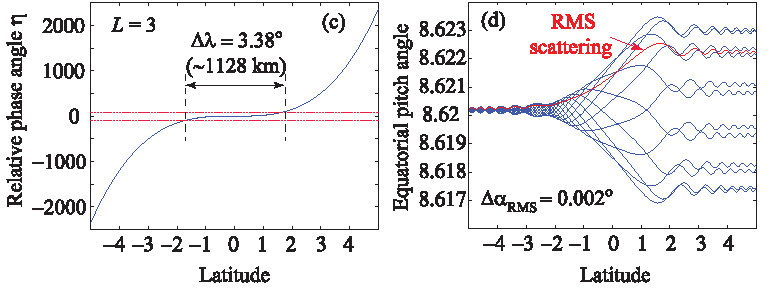
\includegraphics{figures/Bortnik_RMS_scattering.pdf}
\caption[RMS pitch angle scattering from a test particle simulation]{Comparison of RMS and peak deflection in pitch angle from a test particle simulation. On the left is shown the relative gyrophase angle, which must be constant in order for changes to accumulate. On the right is the pitch angle of an array of particles, each with a different initial gyrophase. After the interaction has occurred, the perturbed pitch angles are symmetric about the initial pitch angle. The red curve shows the RMS change. Figure taken from \cite{Bortnik2006}, Figure 7.}
\label{fig:test_particle_sims}
\end{center}
\end{figure}

From here, we follow the numerical solution method from \cite{Bortnik2005, Bortnik2006}. 

A key assumption in our scattering calculation is that the interactions on a single particle from each discrete frequency are independent from one another. Furthermore, we discretize each fieldline into 1$^\circ$ segments, and assume the scattering within each segment is independent from each other. While neither of these assumptions are exactly true, together they provide a critical and substantial reduction in complexity: we no longer have to track the action of the entire set of waves on a discrete set of particles (as in a test particle simulation such as \cite{Chang1985}), but rather can track the stochastic pitch-angle change on a distribution of particles. Additionally, by assuming incoherent scattering across frequencies, the problem becomes much more well-suited to a parallel processing solution, as we can spread computation for each frequency across an array of nodes.\footnote{The coherent-incoherent assumption is based on test particle simulations such as \cite{Chang1985} and \cite{Ristic1993}; however a modernized test-particle (time domain) validation of the approach would be an excellent opportunity for future work!}

Thus, for each set of guide rays $F$, using the interpolation scheme from section \ref{chapter:power}, we can calculate $\Delta \alpha_{RMS}$ as a function of magnetic fieldline, particle energy, and time; the effective change in pitch angle is then determined by summing over the set in quadrature: 
\begin{equation}
\Delta \alpha(E, \vec{x}, t) = \frac{1}{2}\sqrt{\sum_{F} \Delta \alpha_{RMS}^2(E, \vec{x},t, F)}.
\end{equation}

The decision to calculate RMS pitch-angle scattering versus a full test-particle approach is the fundamental difference between \cite{Lauben1998} and \cite{Bortnik2005}, the two most-closely related works to ours. \citeauthor{Bortnik2005} uses the above method, while \citeauthor{Lauben1998} infers expected distributions from a set of test particles. 

As noted by \cite{Lauben1998} and \cite{Lauben2001}, a subset of particles, when subjected to ideal conditions, can ``ride'' a perturbing wavefront across several degrees in latitude, and experience sustained, coherent perturbation. These particles would then precipitate very deeply into the ionosphere, which may account for the lowest-altitude ionization as measured using VLF sub-ionosphere sensing. However these particles represent only a small fraction of the precipitating electrons, the bulk of which experience a random walk through the set of perturbing waves, and are well-modeled by the stochastic RMS formulation of \citeauthor{Bortnik2005}.

\citeauthor{Bortnik2005} makes several approximations which allow for quick numerical integration of \eqref{eqn:bell_dadt_with_labels}, the details of which are beyond the scope of this dissertation. For a concise description of the methodology, see \cite{Bortnik2006}. Table \ref{alg:RMS_change} shows the algorithm in pseudocode. Using the assumptions of incoherence described above, we can independently calculate squared pitch-angle change for every enumerated combination of: a) guide ray sets $F$, b) latitudes along an output fieldline $\lambda$, c) time steps $t$, d) resonant modes $m$, and e) resonant particle energies $E$. 

\begin{algorithm}[t]
\caption{RMS change in pitch angle}\label{alg:RMS_change}
\begin{algorithmic}[1]
\ForAll{output field lines}
	\State{d$\alpha$\_N $\gets$ Zeros(E, t)}\Comment{Pitch angle change at northern hemisphere}
	\State{d$\alpha$\_S $\gets$ Zeros(E, t)}\Comment{Pitch angle change at southern hemisphere}
	\ForAll{sets of guide rays}
		\State{Scale input energy according to input flash location and frequency}
		\ForAll{latitudes along field line $\lambda$}
			\ForAll{time steps $t$}
				\ForAll{resonant modes $m$}
					\State{Calculate $V_{res}$, $E_{res}$}
					\ForAll{grid energies within resonance band $E$}
						\State{$\Delta \alpha_{cur} \gets \int_{t1}^{t2} \frac{d\alpha}{dt}$}
						\State{tN $\gets$ t + $\tau_{f,N}$} \Comment{flight time to northern ionosphere}
						\State{tS $\gets$ t + $\tau_{f,S}$} \Comment{flight time to southern ionosphere}
						\State{d$\alpha$\_N[E, tN] += $(\Delta \alpha_{cur})^2$}
						\State{d$\alpha$\_S[E, tS] += $(\Delta \alpha_{cur})^2$}
					\EndFor
				\EndFor
			\EndFor
		\EndFor
	\EndFor
	\State{d$\alpha$\_N $\gets \sqrt{\mathrm{d}\alpha\_\mathrm{N}}$}
	\State{d$\alpha$\_S $\gets \sqrt{\mathrm{d}\alpha\_\mathrm{S}}$}
\EndFor
\end{algorithmic}
\end{algorithm}


To account for variation in precipitation time, we record the perturbation in pitch angle at the time in which a perturbed particle would precipitate into the atmosphere. This time is dependent on both particle energy and the latitude along the field line where the perturbation occurred, and may be asymmetric between the northern and southern hemispheres.

We compute the time of flight from the interaction latitude $\lambda$ to the ionosphere by assuming a perturbed particle continues along a fixed fieldline, by numerically evaluating the expression from \cite{Walt1994}, equation 4.25:

\begin{equation}
\tau_f =  \frac{1}{v} \int_{s_1}^{s_2} \bigg(1 - \frac{B(s)}{B_{eq}}\sin^2\alpha_{eq}\bigg)^{-1/2} \mathrm{d}s
\label{eqn:bounce_time}
\end{equation}

\subsection{Example energy-time spectra}
Figure \ref{fig:dA_spectra} shows a typical pitch-angle scattering matrix, as a function of electron energy and time delay from a lightning flash at $35^\circ$ latitude, with $I_0=-10$kA. A similar scattering matrix must be computed for every point in the output space (L-shell and longitude offset).

\begin{figure}[h]
\begin{center}
\includegraphics{figures/dA_E-t_spectra.png}
\caption[Pitch angle scattering matrix for a flash at 35$^\circ$ latitude and L=3]{Pitch angle scattering matrix along a fieldine with L=3, for a 10 kA flash at 35$^\circ$ latitude, through a nightside ionosphere at \kp{}=0. Scattering is centered directly over the input flash longitude, within a width of $\pm0.25^\circ.$}
\label{fig:dA_spectra}
\end{center}
\end{figure}

Several key features are apparent: First, the descending curve shape is due to the time delay from the interaction region to the precipitation altitude, with slower moving electrons taking longer to reach the ionosphere. Two banded structures are visible with respect to energy: the dominant band, below $E \sim 10$ keV, is due to the 0-order resonance mode. The upper band with energies above $E  \sim 100$ keV, is due largely to the $\pm$ 1 resonance modes. Scattering efficiency decreases with increasing resonance order, due to the presence of order number $m$ in the denominator of equation \eqref{eqn:bell_dadt_with_labels}, term T1. While some asymmetry exists between the northern and southern hemispheres, the magnitude remains similar due to the numerous bounces of the incident waves, and because the higher-order modes resonate with particles traveling in either direction.

Perturbations in pitch angle due to LEP are generally small; well below $0.1^\circ$. However, due to the exponentially-increasing density of the ionosphere within our precipitation region ($\sim 85 - 100 $ km altitude), and thus the very small change in reflection altitude required, small changes in pitch angle can greatly increase an electron's likelihood of precipitating. Figure \ref{fig:pitch_angle_vs_altitude}(a) shows the perturbed reflection altitudes versus L-shell, for an array of $\Delta \alpha$ values. Figure \ref{fig:pitch_angle_vs_altitude}(b) shows the minimum perturbation value required in order for a particle to reflect at a given altitude.

\begin{figure}[t]
\begin{center}
\includegraphics{figures/pitch_angle_vs_depth.pdf}
\caption[Reflection altitudes vs L-shell for a set of pitch angle perturbations]{(a) Reflection altitude vs L-shell for a particle, for an array of equatorial pitch-angle perturbations. (b) The minimum perturbation required to drive a particle with pitch angle $\alpha = \alpha_{lc}$ to a fixed reflection altitude, as a function of L-shell, for an array of target altitudes.}
\label{fig:pitch_angle_vs_altitude}
\end{center}
\end{figure}


\section{Calculating flux from pitch-angle perturbations}
\label{section:flux_from_pitch_angle}
We have now computed the RMS change in pitch angle along a single field line, as a function of electron energy and time, for a single lightning flash. Next we must convert our scattering matrices (Figure \ref{fig:dA_spectra}) into electron fluxes (or energy fluxes). Again, we follow the method used by \cite{Bortnik2005} (section 5.1.3).

Along each target fieldline, we use our calculated pitch angle changes $\Delta \alpha(E,t)$ to perturb a collection of electrons with an assumed distribution in pitch angle. Perturbation is accomplished by convolving an assumed distribution of particles $G(E,t,\alpha)$ with the perturbing function $\Delta \alpha(E,t)$ for each energy and time bin. The resulting particle flux is the number of electrons within the loss cone ($\alpha < \alpha_{lc}$) after perturbation. We assume that scattering is independent with respect to both the time and energy axes, and can thus be evaluated independently for each $E-t$ bin. Solving the convolution analytically greatly improves computational efficiency.

We use the solution from \cite{Bortnik2005} for a ``ramp'' distribution in pitch angle, which can be applied to any general pitch angle distribution by computing a series approximation about $\alpha = \alpha_{lc}$.

%\begin{equation}
%% Bortnik figure 5.8, equation d.  
%% Maybe you should include a figure here too?
%\end{equation}
%

\begin{figure}[t]
\begin{center}
\includegraphics{figures/da_dist_and_pdf.pdf}
\caption[Pitch angle perturbation vs gyrophase, and corresponding PDF]{(a) Pitch angle perturbation vs particle gyrophase, with $\Delta \alpha_{rms}$ marked, and (b) The corresponding probability density function (PDF, equation \eqref{eqn:pdf}). Modified from \cite{Bortnik2005}, Figure 5.8.}
\label{fig:da_vs_eta_and_pdf}
\end{center}
\end{figure}

\begin{figure}[h]
\begin{center}
\includegraphics{figures/da_dist_and_perturbation.pdf}
\caption[Perturbed pitch-angle distribution]{(a) The initial pitch-angle distribution function and its linear expansion at $\alpha = \alpha_{lc}$. (b) The perturbed distribution, resulting from the convolution of plot (a) with \ref{fig:da_vs_eta_and_pdf}(b). The shaded region indicates particles which have been pushed into the loss cone ($\alpha < \alpha_{lc}$). Modified from \cite{Bortnik2005}, Figure 5.8.}
\label{fig:da_dist_and_perturbation}
\end{center}
\end{figure}

Implicit in this calculation is the distribution in gyrophase, which is taken to be uniform. This allows us to use our RMS pitch angle perturbations in place of an explicit distribution of perturbations across gyrophase. Figure \ref{fig:da_vs_eta_and_pdf} (a) shows the assumed pitch-angle perturbation as a function of gyrophase, $\eta$, and $\Delta \alpha_{RMS}$. We then convert this distribution to its cumulative distribution function F$(\alpha)$, and its probability density function $f(x)$, shown in Figure \ref{fig:da_vs_eta_and_pdf} (b):

\begin{eqnarray}
F(\alpha) & = & P(X < \alpha) = \int_{-\infty}^\alpha f(x) dx \nonumber \\
& = & P((\Delta \alpha_{peak}\sin Y) < x) \nonumber \\
& = & P(Y < \arcsin(x/(\Delta\alpha_{peak})) \nonumber \\  
& = & \frac{\arcsin(\alpha/(\Delta\alpha_{peak}))}{\pi} + \frac{1}{2}  \\
 f(x) & = & \frac{\mathrm{d}F(\alpha)}{\mathrm{d}x} = \frac{1}{\pi\sqrt{(\Delta \alpha_{peak})^2 - (\alpha)^2}}
 \label{eqn:pdf}
\end{eqnarray}

While $\Delta \alpha(E,t)$ is computed only for particles at the edge of the loss cone, $\alpha = \alpha_{lc}$, we note that the perturbation varies slowly with respect to initial pitch angle, and that only particles within $\sim 0.1^\circ$ of the loss cone will be scattered into the loss cone, and can therefore apply the same perturbation to the distribution of electrons just inside the loss cone.

The unperturbed particle population is modeled by:
\begin{equation}
G(E,t,\alpha) = G_1(E, t_0)G_2(\alpha)
\label{eqn:background_density}
\end{equation}
where $G_2(\alpha)$ is the dependence on pitch angle, and $G_1(E, t_0)$ is the energy-differential electron flux at the equator for a given energy band $E$, and time of day $t_0$, along the target field line.

We model $G(\alpha)$ with a sinusoidal distribution between $\alpha=\alpha_{lc}$ and $\alpha = \pi - \alpha_{lc}$, as in Figure \ref{fig:pitchangledistributions}. The background radiation belt density $G(E,t_0)$ is modeled using the AE8 numerical model for both maximal and minimal filling, as in Figure \ref{fig:AE8_model}.

The perturbed flux density $\Phi(E,t,\alpha)$ is given by convolving equations \eqref{eqn:pdf} and \eqref{eqn:background_density}:
\begin{equation}
\Phi(E,t,\alpha) = f(\alpha)*G(E,t,\alpha)
\label{eqn:convolution}
\end{equation}

\begin{figure}[ht]
\begin{center}
\includegraphics{figures/phi_E-t_spectra.png}
\caption[Precipitating flux density E-t spectra for $\lambda_s=35^\circ$ and L=3]{Precipitating flux density $\Phi(E,t)$ along a fieldine with L=3, for a 10 kA flash at $\lambda_s=35^\circ$ latitude, through a nightside ionosphere at \kp{}=0. Scattering is centered directly over the input flash longitude, within a width of $\pm0.25^\circ.$}
\label{fig:phi_E-t_spectra}
\end{center}
\end{figure}

Equation \eqref{eqn:convolution} is evaluated analytically using a linear expansion of $G(E,t,\alpha)$ about $\alpha = \alpha_{lc}$ (\cite{Bortnik2005}, Figure 5.8, section d).

%The resulting convolution gives a perturbed distribution of pitch angles for each energy band $f_\mathrm{p}(E,t,\alpha)$, a portion of which is within the loss cone. To convert the loss-cone pitch angle distribution to a number (or energy) electron flux density $\Phi_\mathrm{p}(E,t,\alpha)$, we apply the formula from \cite{Chang1983}:
%
%\begin{equation}
%\Phi_\mathrm{p}(E,t,\alpha) = \frac{f_\mathrm{p}(E,t,\alpha)v^2}{m \gamma^3}
%\end{equation} 
%
%where $v$, $\gamma$, and $m$ are the velocity, Lorentz correction factor, and mass of a particle. 
Total fluxes are derived by integrating over the loss cone solid angle, again following \cite{Bortnik2005}, including a $\sin^{-2}\alpha_{lc}$ term to account for fieldline focusing, and $\cos\alpha$ to select the plane perpendicular to $B_0$:

\begin{eqnarray}
\Phi(E,t)& = &\frac{1}{\sin^2\alpha_{lc}}\int_0^{2\pi}\int_0^{\alpha_{lc}}\Phi_\mathrm{p}(E,t,\alpha) \cos\alpha \sin\alpha\,d\alpha\,d\phi \\
&=& \frac{1}{\sin^2\alpha_{lc}} \int_0^{\alpha_{lc}}\Phi_\mathrm{p}(E,t,\alpha) \sin 2\alpha\,d\alpha
\label{eqn:phi}
\end{eqnarray}

Figure \ref{fig:phi_E-t_spectra} shows an example $\Phi(E,t)$ matrix, as calculated with a 10-kA flash at $\lambda_s=35^\circ$, for L=3.


Finally, number flux N and energy flux Q can be calculated by integrating over a desired energy band of interest ($E_1, E_2$):

\begin{eqnarray}
N(t) &=& \int_{E_1}^{E_2} \Phi(E,t)\,dE \\
Q(t) &=& \int_{E_1}^{E_2} E \Phi(E,t)\,dE
\end{eqnarray}



\section{LEP stencils and the behavior of a single flash}
\label{section:lep_stencils}
Having developed a method of computing the precipitating electron energy-time spectrum along a single fieldline, we can compute the global precipitation flux due to terrestrial lightning, using a similar ``stencil'' structure as in Chapter \ref{chapter:power}. We then sum over the time axis to compute the electron flux density in equation \eqref{eqn:phi} for each flash, repeating the calculation for a grid of output L-shells and longitudes, for an array of input latitudes, MLT, and \kp{}.

Table \ref{tab:stencil_params} lists the various parameters used in the stencil simulation. The collection of guide rays are the same as those in chapter \ref{chapter:power}.


\begin{table}[t]
\caption{Stencil Simulation Parameters}
\begin{center}

\begin{tabular}{c|c}
Grid and Interpolation Parameters: \\
\hline \hline
Fine-scale Frequencies & 50 \\
Output L-shell range & 1.2 - 8 \\
Output L-shell spacing & 0.2 \\
Output longitude offsets & \{0, 0.5, 1, 1.5, 2, 5, 10, 20\} \\
Threshold distance from flash & 1000 km \\
 & \\
Resonant Interaction Parameters: \\
\hline \hline
Fieldline latitude spacing & 1$^\circ$ \\
Resonant modes & \{ -5 .. 5 \} \\
Energy bands & 256, log-spaced between 10 eV and 10 Mev\end{tabular}
\end{center}
\label{tab:stencil_params}
\end{table}%

After integrating over the time axis, the resulting stencils each have dimensions (lat $\times$ lon $\times$ energy), for both the northern and southern hemispheres. Figure \ref{fig:precip_stencils} shows a set of energy-integrated number flux stencils for a variety of input latitudes and \kp{} for a 10kA, nightside flash. Figure \ref{fig:precip_stencils_day} shows the corresponding stencils for the dayside.

\begin{figure}[]
\begin{center}
\includegraphics{figures/energy_stencils_nightside_v2.png}
\caption[Precipitating flux density stencils for a range of input latitudes and magnetospheric conditions (nightside)]{Precipitating energy density stencils from a maximally-populated radiation belt model, for a range of flash latitudes and magnetospheric conditions, for a 10 kA nightside flash. The location of the plasmapause is marked with a dashed white line, along the northern and southern hemispheres. The flash location is marked with a white X.}
\label{fig:precip_stencils}
\end{center}
\end{figure}

\begin{figure}[]
\begin{center}
\includegraphics{figures/energy_stencils_dayside_v2.png}
\caption[Precipitating flux density stencils for a range of input latitudes and magnetospheric conditions (dayside)]{Precipitating energy density stencils from a maximally-populated radiation belt model, for a range of flash latitudes and magnetospheric conditions, for a 10 kA dayside flash. The location of the plasmapause is marked with a dashed white line, along the northern and southern hemispheres. The flash location is marked with a white X.}
\label{fig:precip_stencils_day}
\end{center}
\end{figure}

By integrating over latitude and longitude, we can compute the total energy precipitated from a single flash, as shown in Figure \ref{fig:total_energy_per_stencil}. A 10-kA flash precipitates on the order of 1 to 10 kJ on the nightside, and 1 to 1000 J on the dayside.

\begin{figure}[]
\begin{center}
\includegraphics{figures/total_energy_vs_latitude.pdf}
\caption[Total precipitated energy for a single flash]{Area-integrated precipitation for a single 10 kA flash vs flash latitude, for a variety of magnetospheric conditions. Totals include precipitation in both hemispheres.}
\label{fig:total_energy_per_stencil}
\end{center}
\end{figure}

Several trends are apparent in figures \ref{fig:precip_stencils} and \ref{fig:precip_stencils_day}: First, it is apparent that increased \kp{} has little impact on precipitation, up until high activity (\kp{}$ > \sim 6$). We can attribute this to our plasmasphere density model, which is consistent across \kp{} values within the plasmapause. Generally, if a flash is launched within the plasmapause (at a latitude lower than that of the plasmapause), then the rays experience relatively little attenuation due to Landau damping in the cold medium, and reflect back and forth several times. Rays launched outside the plasmapause are attenuated much more quickly. The sharp gradient of the plasmapause constrains energy within the plasmasphere, as indicated by the sharp dropoff of precipitation around the plasmasphere latitude. At the highest values of \kp{}, the plasmapause is brought in to L $\sim 2$, about 45$^\circ$, at which point substantial energy is launched outside the plasmapause (and quickly damped), or is very strongly deflected by the plasmapause gradient. The effect of the plasmapause is consistent in both the nightside and dayside stencils.

Examining the dayside stencils in Figure \ref{fig:precip_stencils_day}, the increased attenuation of the ionosphere becomes apparent, notably at lower-latitude flashes. The effect of both ionosphere attenuation and of the lower-latitude plasmapause is apparent when looking at the integrated totals in Figure \ref{fig:total_energy_per_stencil}.

Precipitation is not always symmetric between the northern and southern hemispheres. We can attribute any asymmetry in total flux to the relative efficiency of each resonant mode. Higher-order modes (m = $\pm 1$, $\pm 2$...) are symmetric, with the positive calculation resonating with particles moving in one direction, and the negative with particles moving in the opposite. However, the lowest resonant mode (m = 0) interacts only with counterstreaming particles. Accordingly, precipitation is strongest at the same hemisphere as the incident flash.

In both figures \ref{fig:precip_stencils} and \ref{fig:precip_stencils_day}, precipitation is strongest along a $\sim 0.8^\circ$ offset in longitude, which results from the $\sin^2\theta$ term in equation \eqref{eqn:farfield_power_fd}. In this case, $\theta$ represents the elevation angle from the flash to the lower ionosphere (taken to be 100 km), which is maximized at $\theta = 45^\circ$. The result is a central null in radiated energy directly above the flash, and maximal radiated energy offset by 100 km in the longitudinal direction.

An additional point of interest is the ratio of precipitated energy in Figure \ref{fig:total_energy_per_stencil} vs the radiated energy above the ionosphere in Figure \ref{fig:illumination_totals}. Radiation on the order of megajoules will induce precipitation several orders of magnitude lower in energy. 

Finally we can examine the energy spectrum of precipitating electrons, as shown in Figure \ref{fig:stencil_energy_spectrum}. As in the precipitation stencil maps, increasing \kp{} has little effect until very active conditions. The flux is dominated by lower-energy electrons, owing to the stronger scattering of the lowest resonant mode (also visible in Figure \ref{fig:phi_E-t_spectra}).

\begin{figure}[t]
\begin{center}
\includegraphics[clip]{figures/stencil_energy_spectrum.pdf}
\includegraphics[clip]{figures/stencil_energy_spectrum_AE8MIN_flux_0.pdf}
\caption[Energy spectrum of LEP stencils]{Energy spectrum of precipitating electrons, for \kp{}= 0 and 8, for a range of input latitudes, for day and night. Fluxes are drawn from the AE8MAX population model in the top row, and from the AE8MIN population model in the bottom row.}
\label{fig:stencil_energy_spectrum}
\end{center}
\end{figure}


\section{Coordinate deformation}
The stencils in section \ref{section:lep_stencils} are computed using a dipole magnetic field, and the simplified GCPM model, both to reduce computational complexity and to better generalize to multiple longitudes. However, we can approximate the effect of a more-complex magnetic field model via a coordinate transformation, in which we rotate input coordinates to an equivalent dipole-model coordinate, and perform an inverse operation on the stencil output. On the stencil output, this approximation is justified by noting that trapped electrons are bound to their respective field lines, regardless of model used. Justification on the input side (deforming the input coordinates of a lightning flash) is less-concrete, but still a reasonable assumption. First, experimentation with the raytracer reveals that, given a longitudinally-symmetric plasma density model, rays generally follow the longitude deviation of the magnetic field model. Second, while the IGRF and Dipole models differ greatly in its footprint on the ground (as in Figure \ref{fig:Lshell_example}), within the plasmasphere the two models have reasonable agreement (as in Figure \ref{fig:fieldline_example}).

The \emph{Corrected Geomagnetic Coordinate} (CGM) \citep{Hakura1965} system is especially well-suited for this task. CGM coordinates are defined by fieldline tracing between the IGRF and Dipole models. To transform from geographic to CGM coordinates, we first trace a fieldline using IGRF from the surface, up to its intersection with the geomagnetic equatorial plane. We then follow the dipole model back down to the surface, to get an equivalent dipole-model coordinate. The inverse transformation is accomplished by following the dipole field line back up to the equator, and the IGRF model down to its footprint \citep{Laundal2016}.

Field line tracing is a computationally-intensive task for a coordinate transformation tool. Historically, researchers relied on precomputed lookup tables and interpolation. The Altitude-Adjusted CGM (AACGM) model \citep{Baker1989, Shepherd2014} uses a spherical-harmonic fit to rapidly transform between CGM and MAG coordinates.

\begin{figure}[t]
\begin{center}
\includegraphics{figures/CGM_globe_comparison.pdf}
\caption[Comparison of Magnetic Dipole (MAG) and Corrected Geomagnetic (CGM) coordinates]{A comparison between Magnetic Dipole (MAG) and Corrected Geomagnetic (CGM) coordinates. Corrected Geomagnetic coordinates are obtained by following a magnetic field line, as defined by IGRF, from an input point to its intersection with the magnetic dipole equator. The CGM latitude and longitude are then obtained by following the dipole field line to its footprint on the Earth's surface. Contours are spaced every $20^\circ$ in geomagnetic latitude, and $30^\circ$ in geomagnetic longitude.}
\label{fig:CGM_globe_comparison}
\end{center}
\end{figure}    

CGM coordinate systems are undefined at some regions near the geomagnetic equator, due to the fact that some IGRF fieldlines may never intersect with it. In these cases, approximate models are often used. \cite{Baker1989} simply omitted geomagnetic latitudes within $\sim 24^\circ$ of the equator from their study; subsequent researchers have performed spline fits and interpolation to further reduce the undefined region.

We use the AACGMv2 algorithm and implementation from \cite{Shepherd2014}, available at \emph{http://superdarn.thayer.dartmouth.edu/aacgm.html}. Figure \ref{fig:CGM_globe_comparison} compares MAG and AACGM contours on a geographic map.

Figure \ref{fig:CGM_vs_MAG_GLD} shows the relative difference between GLD average current density using MAG coordinates only, vs using the AACGM coordinate transform.



\begin{figure}[]
\begin{center}
\includegraphics{figures/GLD_CGM_vs_MAG_comparison.png}
\caption[GLD average peak current density, adjusted using AACGM coordinates]{Average lightning activity, weighted by peak current intensity, as measured by the GLD360 dataset. Data is averaged from August 2014 through July 2017. (a) the GLD360 data, in geographic coordinates. (b) the GLD360 data, shifted to its equivalent coordinates using the AACGM coordinate transform. (c) the relative error between the two coordinate frames.}
\label{fig:CGM_vs_MAG_GLD}
\end{center}
\end{figure}


% Our study already excludes these latitudes on the basis that below $\sim 20^\circ$ geomagnetic latitude, field lines do not exit the ionosphere at their apex.


\section{Global and Seasonal Energy Fluxes}

Having computed the precipitation for a single flash across a variety of input parameters, we can examine global energy deposition by shifting, scaling, and summing the LEP stencils according to the GLD360 lightning dataset. The resulting electron precipitation is heavily dependent on the population of radiation belt electrons; we provide two estimates, using the AE8 model for maximal and minimal filling, in effort to determine the upper and lower bounds on precipitation. \footnote{An interesting opportunity for future work would be to incorporate historical data, as filling events and \kp{} activity are likely correlated.}

LEP stencils are computed using the parameters in table \ref{tab:stencil_params}. Stencils are computed for canonical 10 kA flashes, in 5$^\circ$ steps in latitude, between 15$^\circ$ and 55$^\circ$, for dayside and nightside (MLT = 12 and 0 respectively), for an array of \kp{} = \{0, 2, 4, 6, 8\}. The resulting stencils are then interpolated onto a fixed 0.5$^\circ$x0.5$^\circ$ grid in geomagnetic latitude and longitude, and for all valid values of \kp{} (0 - 9 in $\sim$ 0.3 steps). Noting the relatively quick transition at the day/night terminator, we bin each flash in the GLD360 dataset into dayside or nightside. The 256 energy bands are summed into 64 sub-bands to reduce memory requirements. 

Figure \ref{fig:global_precip_map_max_min} shows the global average energy precipitation resulting from LEP, for maximum and minimum conditions. Precipitation is integrated over the energy band of interest (10 eV - 10 MeV), and averaged over a three year period between August 2014 and July 2017. We use historical data for \kp{}, which is reported in three-hour segments.

The pitch-angle scattering model scales linearly with respect to wave amplitude, and therefore scales quadratically with respect to flash peak current. To account for arbitrary peak current values, we scale the resulting precipitation stencils accordingly:

\begin{equation}
\phi(I) = \phi(I_{ref})\frac{I^2}{I_{ref}^2} 
\end{equation}

The two sources of stochasticity in our model are 1) the location and intensity of lightning, and 2) the value of \kp{}. Lightning activity and \kp{} are generally uncorrelated, as \kp{} is driven by activity within the magnetosphere, and lightning activity by terrestrial weather patterns. As shown in figures \ref{fig:precip_stencils} and \ref{fig:precip_stencils_day}, fluctuations in \kp{} have little effect on our precipitation model in most situations (\kp{}$ < 6$). Unexplored in this work, however, is the correlation between radiation belt filling conditions and \kp{}; e.g., radiation belt filling events generally occur alongside geomagnetically-active conditions, in which \kp{} will be high.

\begin{figure}[]
\begin{center}
\includegraphics{figures/global_precip_map_max_min.png}
\caption[Global energy deposition ``hot spots'' for maximal and minimal radiation belt populations]{Time-averaged energetic electron precipitation ``hot spots'', for the GLD360 dataset, between August 2014 and July 2017. Total energy is shown, integrated between 10 eV and 10 MeV. }
\label{fig:global_precip_map_max_min}
\end{center}
\end{figure}

By integrating over latitude and longitude, rather than time, we can examine any seasonal trends which may be present. Figure \ref{fig:seasonal_precip_rates_global} shows the global energy flux in kilowatts, across the globe, as a function of time, for maximal and minimal filling conditions. The global energy deposition rate shows very weak seasonal dependence, and can range from a few kilowatts to several megawatts. The disperse energy deposition rate suggests that LEP is not a prominent driver of energy in the upper atmosphere. However, sporadic energy deposition due to LEP is measurable by sub-ionosphere VLF remote sensing \citep{Inan1990, Johnson1999, Cotts2011}, and may still be capable of inducing turbulence in the upper ionosphere, either by precipitating particles or the interaction of the upgoing whistler wave \citep{Berthelier2008}.

The lack of seasonal dependence, however, suggests that LEP can provide a constant, year-round loss mechanism for radiation belt electrons, especially when considering that radiation belt electrons can drift in longitude around the Earth, on timescales of minutes to days \citep{Walt1994}, and can thereby interact with lightning activity across the globe.

\begin{figure}[ht]
\begin{center}
\includegraphics{figures/seasonal_precip_rates_global.pdf}
\caption[Global energy deposition due to LEP]{Global average energy deposition due to LEP. Precipitation is integrated across the globe, for energetic electrons between 10 eV and 10 MeV.}
\label{fig:seasonal_precip_rates_global}
\end{center}
\end{figure}
\begin{figure}[h]
\begin{center}
\includegraphics{figures/seasonal_precip_rates_US_only.pdf}
\caption[Global energy deposition due to LEP over the continental United States]{Average energy deposition due to LEP over the continental United States (20$^\circ$ to 50$^\circ$ geomagnetic latitude, -50$^\circ$ to +10$^\circ$ geomagnetic longitude). Seasonal variation is much more apparent than in the global integration (Figure \ref{fig:seasonal_precip_rates_global}).}
\label{fig:seasonal_precip_rates_US_only}
\end{center}
\end{figure}

While total global lightning activity is relatively constant, regional lightning is a highly seasonal phenomenon. We can integrate the energetic electron precipitation over the continental United States, to explore seasonal dependence on a finer scale, such as in \cite{Gemelos2009}. Figure \ref{fig:seasonal_precip_rates_US_only} shows the total energy precipitation between 20$^\circ$ - 50$^\circ$ in geomagnetic latitude, and -50$^\circ$ to +10$^\circ$ in geomagnetic longitude (approximately over the continental United States). Narrowing our observation window reveals a much greater seasonal variation, peaking in the summer months, and reaching a minimum in December and January.



\section{Lifetime Estimates}
The previous section examined the energy deposition into the ionosphere due to LEP. Next, we consider the relative effect of LEP as a loss mechanism from the populated radiation belts.

Our precipitation model is linearly proportional to the current population of electrons along a given magnetic fieldline, which results in an exponential loss function, parameterized by a time constant $\tau$:

\begin{eqnarray}
\frac{dN}{dt} & \propto & N \\
\therefore N(t) & = & N_0 \exp{-t/\tau} \\
\frac{dN}{dt} & = & -\frac{N_0}{\tau}\exp{-t/\tau} \\
& = & -\frac{N(t)}{\tau} \\
\tau & = & \frac{N(t=t_0)}{dN/dt\rvert_{t0}}
\label{eqn:tau}
\end{eqnarray}

Once summed over the GLD360 dataset, our model delivers electron losses impinging on a cross-sectional area at 100 km, with units [$\#$/cm$^2$/eV/sec]. To compute the percentage loss, we must determine the number of electrons (per energy) which occupy the fieldline above the same cross-sectional area, resulting in $\tau \sim sec$.

The total electrons along a given fieldline above a cm$^2$ ionosphere patch is computed by integrating the (energy) differential, omnidirectional equatorial flux, such as from the AE8 model. As in the precipitation code, we ascribe a sinusoidal pitch-angle distribution (e.g., Figure \ref{fig:pitchangledistributions}) to the electrons in the omnidirectional flux value. 

The AE8 energy-differential, omnidirectional flux models deliver data with units J $\sim$ [$\#$/cm$^2$/sec/ev], representing the total flux of electrons through a cross-sectional area at the equator, per unit energy. We use a change of variables and integrate over the sinusoidal pitch-angle distribution P(L, $\alpha$), using the relationship in equation \eqref{eqn:bounce_time} to relate an electron's bounce time $\tau_b$ to it's pitch angle $\alpha$ and total kinetic energy $E$.

\begin{equation}
  P(L,\alpha)=\begin{cases}
    \bigfrac{1}{1 - 2\alpha_{lc}/\pi}\sin{\bigfrac{\alpha - \alpha_{lc}}{1 - 2\alpha_{lc}/\pi}}, & \text{$\alpha_{lc} < \alpha < \pi - \alpha_{lc}$}. \unit{rad^{-1}}\\
    0, & \text{otherwise}.
  \end{cases}
\end{equation}


\begin{equation}
 % There's more to this -- I'm not showing the whole integrand after the change of variables and addition of the pitch-angle distribution
N_{0,equator} = \int_0^{\pi/2} J(E)P(L,\alpha) \tau_b(L, \alpha)\,\sin{\alpha}\,\cos{\alpha}\,d\alpha \unit{\#/cm^2/eV}
\end{equation}

We then convert the integrated value $N_0$ from an equatorial cross-sectional area to an equivalent cross-sectional area at the ionosphere, using a ``focusing'' term $C_b$, given by the ratio of cross-sectional areas bounded by a pair of field lines:

\begin{eqnarray}
\epsilon_m &= & \frac{1}{L}(R_E + H_{iono})/R_E \\
C_b & = & \sqrt{1 + 3(1 - \epsilon_m)} / \epsilon_m^3 \\ 
N_{0, iono} &=& C_b\,N_{0, equator} \unit{\#/cm^2/eV}
\label{eqn:fieldline_density}
\end{eqnarray}

In order to examine the effectiveness of LEP across all energies, and avoid numerical issues where the AE8 model values are small, we compute an additional set of stencils, using a uniform radiation belt population, by setting $J(E) = 1$ [1/cm$^2$/sec/ev].  Figure \ref{fig:stencil_energy_spectrum_flat_distribution} shows the precipitated energy distribution from a flat radiation belt population, in the same format as Figure \ref{fig:stencil_energy_spectrum}. The bimodal peaks resulting from the multiple resonant interaction modes are more-readily visible, without the additional loss due to reduced radiation belt populations at higher energies.

\begin{figure}[]
\begin{center}
\includegraphics{figures/stencil_energy_spectrum_flat_distribution.pdf}
\caption[Energy spectrum of LEP stencils, drawn from a uniform radiation belt population]{Energy spectrum of precipitating electrons, for \kp{}= 0 and 8, for a range of input latitudes, for day and night, from a uniform (differential flux = 1/cm$^2$/sec/eV) fieldline population.}
\label{fig:stencil_energy_spectrum_flat_distribution}
\end{center}
\end{figure}

We then compute an equivalent precipitation map using the GLD360 dataset, and the flat-distribution stencils. We average the resulting precipitation over all latitudes to obtain a typical flux estimate. The loss timescale, $\tau$, is then obtained using equation \eqref{eqn:tau}, with the fieldline population $N$ computed using equation \eqref{eqn:fieldline_density}, and the loss rate $dN/dt$ given by the global average precipitation estimate, both using the flat distribution for $J$.

Figure \ref{fig:electron_lifetimes} shows the estimated lifetime for radiation belt electrons, subjected solely to LEP-induced losses, versus electron energy and fieldline. Two prominent results are apparent in Figure \ref{fig:electron_lifetimes}: First, we see two enhancement regions, centered at lower energies ($\sim$100 eV), and at higher energies ($\sim$ 10 MeV). We can attribute this bimodal pattern to the preferential energy bands of each resonant mode, as in Figure \ref{fig:stencil_energy_spectrum_flat_distribution}. Interestingly, our model shows a null in precipitation effectiveness in the band between 100 keV and 1 MeV; this band has generally been thought to be the dominant precipitation region (for example, the analysis of a single LEP event in \cite{Voss1998} shows a precipitation spectrum between $\sim$ 100  -- 300 keV. The instrument used, SEEP, measured fluxes binned into 8 energy channels between 2 keV and 10 MeV.) . Second, LEP is only an effective loss mechanism for inner belt and slot-region fieldlines (L $<$ 3), owing to the much much greater volume traversed by higher-L fieldlines.
\begin{figure}[t]
\begin{center}
\includegraphics{figures/electron_lifetimes_updated_power_with_labels.png}
\caption[Estimated lifetime of radiation belt electrons subject to LEP losses only]{Estimated lifetimes ($\tau$, the time required for a population to decay by 1/e) for radiation belt electrons subjected solely to LEP-induced losses.}
\label{fig:electron_lifetimes}
\end{center}
\end{figure}


\section{Comparison to other research}
We can compare our resulting precipitation estimates to two related works: \cite{Gemelos2009} used data from the DEMETER spacecraft, along with seasonal lightning fluxes as measured by the NLDN network, to examine seasonal trends in LEP at 126 keV, and \cite{Meredith2007}, which uses \emph{in situ} VLF wave measurements to estimate lifetimes of radiation belt electrons due to various scattering mechanisms (LEP, chorus, hiss), using an incoherent interaction model.

Figure \ref{fig:gemelos_comparison} shows our modeled electron precipitation at 123 keV for August and December, averaged over 2014 - 2017, along with the corresponding northern hemisphere lightning activity as measured by GLD360, to facilitate comparison with \cite{Gemelos2009}, Figure 1. Geographically, our model shows very good agreement with \citeauthor{Gemelos2009}; however our modeled fluxes are several orders of magnitude lower. Possible explanations for the discrepancy in precipitation amplitude are that the DEMETER spacecraft orbited at 710 km altitude, while our fluxes are estimated at 100 km. Additionally, the DEMETER particle detector viewed particles with local pitch angles near $\sim 85^\circ$, and a full-width, half maximum viewing angle of $30^\circ$. Both \citeauthor{Gemelos2009} and \cite{Sauvaud2006} state that at this orientation the detector measures particles within or near the \emph{drift} loss cone, which may be considerably shallower than the bounce loss cone as modeled by our work.

\begin{figure}[]
\begin{center}
\includegraphics{figures/Gemelos_comparison.png}
\caption[Precipitation at 123 keV over the continental United States, for summer and winter]{Average precipitation at 123 keV over the continental United States, for summer (August) and winter (December). The bottom plots show the corresponding northern-hemisphere lightning as measured by GLD360.}
\label{fig:gemelos_comparison}
\end{center}
\end{figure}

Figure \ref{fig:Meredith_comparison} compares our estimated electron lifetimes to those reported by \cite{Meredith2007}. \citeauthor{Meredith2007} estimates electron lifetimes using a database of magnetosphere VLF wave measurements from the CRRES spacecraft; they then compute pitch angle scattering using the PADIE code, for a variety of assumed wave conditions. \citeauthor{Meredith2007} concludes that pitch angle scattering due to magnetospherically-reflecting whistlers (e.g., LEP) is of little relevance to relativistic electron lifetimes. However, \citeauthor{Meredith2007} uses an incoherent, quasilinear diffusion model, and therefore may not capture the effects of resonant pitch-angle scattering.

Our work is somewhat consistent, in that within the specified energy band, both works show lifetimes much greater than expected, suggesting that LEP is not a dominant loss mechanism. However, our model does show shorter lifetimes at lower L-shells. Additionally, \citeauthor{Meredith2007} does not examine lifetimes of lower energy electrons, for which our model shows the strongest losses. 
\begin{figure}[]
\begin{center}
\includegraphics{figures/Meredith_comparison_thesis.pdf}
\caption[Electron lifetime estimates compared against \cite{Meredith2007}]{Comparison of estimated electron lifetimes with those of \cite{Meredith2007}. Red lines show our results; blue lines show \cite{Meredith2007} estimates for quiet geomagnetic conditions; and orange for active geomagnetic conditions. Dashed black lines indicate the approximate measured lifetime of electrons (1 to 10 days).}
\label{fig:Meredith_comparison}
\end{center}
\end{figure}



    \chapter{Satellite Instrumentation for LEP Measurement}
    	\section{VPM Mission Overview}
\section{Hardware Architecture}
\subsection{Wave Measurement}
\subsection{Particle Measurement}
\section{Firmware Architecture}




    \chapter{Conclusions}
    	Over the preceding chapters we have examined the global impact of lightning-generated whistlers, and associated electron precipitation, on the ionosphere and radiation belts. 

In Chapter \ref{chapter:power} we modeled the persistent radio energy within the plasmasphere and magnetosphere due to lightning-generated whistlers; the energy is generally confined by the plasmapause, inside which there is little variation with respect to geomagnetic conditions. We find that the persistent energy decays logarithmically with increasing L-shell, as in figure \ref{fig:energy_density_vs_L_trendline}. We find a similar logarithmic trend in the radio frequency spectrum, in which the average bandwidth of lightning-generated energy decreases with increasing L-shell, as in figure \ref{fig:energy_density_vs_L_vs_freq}.

Chapter \ref{chapter:global_estimates} built on the ray tracing and interpolation methodology of Chapter \ref{chapter:power} to examine the global impact of LEP, both as a magnetosphere-ionosphere energy coupling mechanism, and as a radiation belt depletion mechanism. We consider energy deposition from maximally and minimally populated radiation belts. We capture the seasonally-varying morphology of \cite{Gemelos2009}, and are in reasonable agreement with \cite{Meredith2007} for electron average electron lifetimes in the MeV energy range. Our simulation finds that while LEP is not a significant loss mechanism for highly-relativistic electrons in either the inner or outer belts, we find LEP may be a significant loss mechanism for suprathermal (100 eV - 10 keV) electrons in the inner radiation belt. We do not find any notable enhancement in slot-region losses, suggesting that LEP is not significant in the depletion of the slot region. However, we consider only the first 20 seconds of a propagating whistler, after which significant energy in the middle frequencies and middle L-shells remain; as was theorized by \cite{Bortnik2005}, this energy likely evolves into incoherent plasmaspheric hiss, which has been surmised elsewhere to be the principal driver of the slot region.

Chapter \ref{chapter:VPM} detailed the practical issues of a CubeSat-based VLF receiver, designed for \emph{in situ} measurements of LEP. While the receiver was constrained by the power and volume requirements of a CubeSat, this system included additional constraints not normally addressed in microscale / university-level satellite design. These constraints include designing for radiation-tolerant upgrades which while of small significance for short-duration, low-earth-orbit missions, may be of greater significance for highly-elliptical orbits or future CubeSat missions to planets and objects outside the magnetosphere. Additionally, the receiver was designed as a peripheral device, with no volatile software onboard, using the hardware description language VERILOG.

\section{Suggestions for Future Work}

\subsection{Model Improvements}
\paragraph{Ray Tracing}
The morphology of LEP is driven primarily by the paths of incident whistlers; within our modeling, these paths are defined through raytracing in a modeled plasmasphere environment. Numerous improvements could be made here, with possible new science of interest, as the detail and realism in plasmasphere modeling is increased. Driven by both a desire to generalize, and a lack of computational resources, we artificially constrain our raytracing to the meridional plane (as defined by the Earth's magnetic field). Furthermore, we had difficulty in balancing accuracy versus reasonable timestepping (reducing error tolerances would frequently reduce our timestep to picoseconds), which resulted in erroneous deviation along the longitudinal axis. Exploring alternatives to the Runge-Kutta ODE solver, as well as incorporating the warm plasma corrections of 
\cite{Maxworth2017} may serve to reduce these errors.
Generally, at noon and midnight local time, we expect minimal gradients in the zonal direction, and the meridional-plane constraint should hold. However, lightning predominantly occurs around dusk (as in figure \ref{fig:Io_and_MLT}), where there may likely be stronger longitudinal gradients, which could impart a significant spreading or offset to the precipitation stencils of Chapter \ref{chapter:global_estimates}. % different solvers, etc, etc, warm plasma effects, etc etc.

\paragraph{Interpolation and Granularity}
The energy and precipitation stencils could each benefit from a finer granularity in guide rays, and from finer frequency steps in interpolation. An additional, reasonably-straightforward modification to our interpolation scheme would be to consider the \emph{concave hull} mentioned in figure \ref{fig:convex_hulls}. Our interpolation algorithm at present assumes a convex hull, which will always span a volume equal to or greater than the concave hull.

\paragraph{Backscatter and Altitude Effects}
Our precipitation codes do not include the Atmospheric Backscatter model of \cite{Cotts2011}; \citeauthor{Cotts2011} finds that a significant fraction of electrons bounce back after penetrating below 100km altitude (below which our model considers a particle to be lost). The rebounded particles may then interact with additional VLF wave activity, and possibly precipitate into the opposite hemisphere.

Of interest for transmitter-based measurements of LEP would be a more-thorough treatment of precipitating depth. As noted in \cite{Cotts2011}, there is a significant difference in precipitation likelihood between `grazing' precipitation and `deep' precipitation. Furthermore, the lower-energy, suprathermal electrons which comprise the bulk of our precipitation energy estimates likely precipitate at higher altitudes; VLF transmitter remote sensing techniques are sensitive dominantly to the lower edge of the ionosphere ($\sim$ 85 km), and may not be impacted by particles deposited closer to our 100 km threshold.
% raytracer improvements
% Incorporation of Atmospheric Backscatter codes
% Consideration of absorption altitude (low-energy stuff gets driven down *hard*, but always precipitates closer to 100km -- insignificant for transmitter studies?

\subsection{Global Trend Improvements}
\paragraph{Correlation between Filling Conditions and \kp{}}
% Filling conditions -- higher kp = higher filling, but lower wave activity?
The dynamics of the radiation belts are marked by short-duration, sporadic filling events. These filling events may coincide with increased solar activity (possibly with a delay), which in turn may result in a higher \kp{}. Within our work, we consider precipitation from maximally and minimally filled radiation belts. However, we find less precipitation at higher \kp{} values, due to the constricting nature of the plasmapause. Incorporating measured / historical filling data along with GLD360 and \kp{} data may result in a better estimate of energy deposition, rather than an upper or lower bound.

\paragraph{Coherent vs Incoherent Methods}
In Chapter \ref{chapter:global_estimates}, we determine global electron precipitation by taking a scaled sum of individual, (pseudo) coherent precipitation events using GLD360. However, numerous work exists on incoherent diffusion methods \citep{Kennel1966, Lyons1973, Glauert2005}. Rather than summing the precipitation after interaction, one could use the power estimates from Chapter \ref{chapter:power}, and feed the determined distributions into an incoherent diffusion code. Such an implementation would be an excellent comparison between the coherent and incoherent diffusion approaches, which generally treat different physical systems -- coherent for LEP, and incoherent for chorus and hiss.
% Comparison to PADIE codes, etc

\subsection{Related Phenomena}
\paragraph{Cloud-to-Cloud lightning}
Our study is constrained to lightning discharges measured by the GLD360 dataset, which is designed to detect Cloud-to-Ground only. However, Cloud-to-Cloud lightning may be a significant, additional source of whistler waves, and subsequently LEP. The single-flash modeling used in computing the energy and LEP stencils could be easily adapted to model a cloud to cloud discharge; one would need only to provide a new model of illumination (see section \ref{section:input_power}, and a dataset of cloud-to-cloud lightning activity. 
% cloud-to-cloud
\paragraph{Transmitter-induced Precipitation}
Similarly, the stencil computation method could be adapted to study precipitation resulting from VLF transmitters. In contrast to the impulsive, broadband whistlers generated by lightning, VLF transmitters provide a constant, narrowband signal. It has been theorized that the constant effect of numerous global transmitters constitutes an anthropogenic driver of the so-called ``impenetrable barrier'' for relativistic electrons \citep{Baker2014, Foster2016}.
% power and precipitation estimates for VLF transmitters

% different lightning datasets -- detection efficiency?

% Comparison to real data!



   \appendix
   \chapter{Reference Equations}
    \section{Landau Damping}
\label{appendix:landau}

In raytracing, we calculate wave growth and attenuation according to Landau damping. We use the \citet{Brinca1972} formulation -- itself a reorganization of \cite{Kennel1966} -- which assumes a cold background plasma, onto which a small thermal electron population is ascribed. The following (frustratingly complex) equation set is taken from \cite{Brinca1972}, and reprinted here for organization.

Calculating a growth rate begins simply: we assume a time-varying plane wave in the usual complex (``phasor'') form:

\begin{equation}
E \sim E_0 \exp{i(\omega t - \vec{k}\cdot\vec{r})}
\end{equation}

If either $\omega$ or $\vec{k}$ have an imaginary component, then the result will be an additional real-valued term, which we can factor out as $\chi$:
\begin{eqnarray}
E & = &E_0 \exp{i( \omega t - (\vec{k_r} + i\vec{k_i})\cdot\vec{r})} \\
& = &E_0 \exp{-\chi r}\exp{i(\omega t + \vec{k}\cdot\vec{r})}
\end{eqnarray}

If the new exponential term $-\chi$ is positive, the wave will be amplified; if the term is negative, the wave will be attenuated.

The spatial growth rate $\chi$ is given by equation \ref{eqn:brinca_chi} \citep{Brinca1972,Kennel1966}:
\begin{equation}
\chi = -\frac{c k_i}{\omega} = \frac{\delta}{4 \eta (2 A \eta^2 - B)} \big( T_1 - T_2 - T_3 \big) \\ \label{eqn:brinca_chi} 
\end{equation}
with the following terms:

\begin{eqnarray}
&T_1 = & \frac{\eta^2\sin{\theta}^2 - P}{2(S - \eta^2)}\Gamma_I \cdot [(R - \eta^2)J_{m-1} + (L - \eta^2)J_{m+1}]^2 G_1 \\ \nonumber
&T_2 = & 2[(S - \eta^2 \cos^2\theta)(S - \eta^2) - D^2] \Lambda_I J_m G_2 \\ \nonumber
&T_3 = & 2\eta^2 \sin \theta \cos \theta \Gamma_I\cdot [(R - \eta^2)J_{m-1} + (L - \eta^2)J_{m+1}]G_2 \\ \nonumber
\end{eqnarray}

where $\chi > 0$ indicates damping.

Note that \citeauthor{Brinca1972} has related the temporal damping rate $\omega_i$ from \cite{Kennel1966} to a spatial damping rate $k_i$ by assuming a constant propagation at the group velocity $v_g$.

$A, B, C, D, L, P, R,$ and $S$ are the Stix environment parameters given by \ref{eqn:stix_params_1} -- \ref{eqn:stix_params_2}, and are functions of wave frequency, local plasma density, and local magnetic field strength. 

As previous, $\theta$ is the angle between the wavenormal vector and the background magnetic field, and $\eta$ is the wave refractive index, found by solving equation \ref{eqn:disp_rln}.

The terms $J_m, J_{m+1}$ and $J_{m-1}$ are Bessel functions of the first kind, which account for the multiple resonant modes -- $m=0$ indicates the Landau resonance; $m\pm1$ the Cyclotron resonance.

The terms $\Gamma_I$ and $\Lambda_I$ are summations over resonant modes $m\in \{-\infty...\infty\}$ , and integrations over the velocity space $v_\perp$,$v_\parallel$ given by:

\begin{eqnarray}
&\Gamma_I &= \frac{2\pi^2\omega_p^2}{\omega k_\parallel} \sum_{m=-\infty}^{\infty}\int_0^\infty v_\perp^2 dv_\perp \int_{-\infty}^\infty \delta(v_\parallel - V_m) d v_\parallel \\
&\Lambda_I &= \frac{2\pi^2\omega_p^2}{\omega k_\parallel} \sum_{m=-\infty}^{\infty}\int_0^\infty v_\perp dv_\perp \int_{-\infty}^\infty v_\parallel \delta(v_\parallel - V_m) d v_\parallel
\end{eqnarray}
\begin{equation}
V_m = \frac{\omega - m\omega_c}{k_\parallel}
\end{equation}

Finally, the temperature distribution is included in the values $G_1$ and $G_2$ -- each of which are functions of the \emph{gradient} of the phase-space distribution function:

 $f=f(\vec{x}, \vec{v}) = f(\vec{x}, v_\perp, v_\parallel)$:

\begin{equation}
G_1 = \bigg(1 - \frac{k_\parallel v_\perp}{\omega}\bigg)\frac{\partial f}{\partial v_\perp} + \frac{k_\parallel v_\perp}{\omega}\frac{\partial f}{\partial v_\parallel}
\end{equation}
\begin{equation}
G_2 = J_m\bigg[\bigg(1 + \frac{m \omega_c}{\omega}\bigg)\frac{\partial f}{\partial v_\parallel} - m \frac{\omega_c}{\omega v_\perp} \frac{\partial f}{\partial v_\perp}\bigg]
\end{equation}

Despite the complexity of these equations, the phase-space distribution function $f$ is the only fundamental new input -- every remaining parameter is an output of the raytracer, and itself a result of our plasma density and magnetic field models.

Our implementation, derived from \cite{Golden2010}, computes the gradients of $f$ numerically using finite differencing, therefore granting the flexibility to use any arbitrary distribution function.


%& = & \frac{\delta}{4 \eta (2 A \eta^2 - B)} \big\{\frac{\eta^2\sin{\theta}^2 - P}{2(S - \eta^2)}\Gamma_I \\ \nonumber 
    
    \chapter{Runge-Kutta Methods}
    \label{appendix:runge_kutta}

    \bibliography{library}
    \end{document}








 









Documentation: 
    This style file modifies the standard report style to follow the
    Graduate Degree Support Section of the Registrar's Office's
    "Directions for Preparing Doctoral Dissertations".  It sets the
    margins and interline spacing and disallows page breaks at
    hyphens.

    The \beforepreface command creates the title page, a copyright page
    (optionally), and a signature page.  Then the user should put
    preface section(s), using the \prefacesection{section title}
    command.  The \afterpreface command then produces the tables of
    contents, tables and figures, and sets things up to start
    the main body (on arabic page 1).
    
    The following commands can control what goes in the front matter
    material:
    
        \title{thesis title}
        \author{author's name}
        \dept{author's department}
                - Computer Science if omitted
The following switches allow for special title pages (not all are current)
        \committeethesis - for a thesis in a committee (no dept.)
                           use \dept{committee name}
        \programthesis - for a thesis in a program (no dept.)
                           use \dept{program name}
        \educationthesis - for the School of Education. \dept doesn't matter
        \businessthesis - for the GraduateSchool of Business. \dept doesn't matter
        \lawthesis - for the School of law. \dept doesn't matter
        \humanitiesthesis - for a thesis also submitted to the Graduate
                            Program in Humanities
        \specialthesis  - for a Graduate Special thesis
        \industrialthesis - for a thesis in Industrial Engineering
        \dualthesis     - for a thesis in a dual language department.
                          Also define \languagemajor{language}.
                          e.g., \dept{French and Italian} 
                          \languagemajor{Italian}
         \principaladviser{the principal advisor's name}
           (or \principaladvisor, if you prefer advisor spelled with o)
        \coprincipaladviser{optional second principal advisor's name}
           (or \coprincipaladvisor, use only if you have two principal
           advisors only for the second one)
        \firstreader{the first reader's name}
        \secondreader{the second reader's name}
        \thirdreader{optional third reader's name}
        \fourthreader{optional fourth reader's name}
        \setlength{\signaturespace}{.5in} 
                - default is .5in, can be adjusted to fit all
                signatures in one page
        \submitdate{month year in which submitted to GPO}
                - date LaTeX'd if omitted
        \copyrightyear{year degree conferred (next year if submitted
          in Fall quarter)}
                - year LaTeX'd (or next year, in December) if omitted
        \copyrighttrue or \copyrightfalse
                - produce or don't produce a copyright page (true by default)
        \thesiscopyrighttrue or \thesiscopyrightfalse
                - produces the style of copyright page listed by the
                Thesis Office or the style that everyone else uses
                (Thesis office by default).
        \figurespagetrue or \figurespagefalse
                - produce or don't produce a List of Figures page
                  (true by default)
        \tablespagetrue or \tablespagefalse
                - produce or don't produce a List of Tables page
                  (true by default)

This style uses interline spacing that is 1.3 times normal, except
in the figure and table environments where normal spacing is used.
That can be changed by doing:
    \setstretch{1.6}
(or whatever you want instead of 1.6)

This command should be put before the \begin{document} command but
after loading the packages

You can also set any particular section in singlespacing mode by using
the singlespace environment.  For example

\begin{quote}
\begin{singlespace}
...
\end{singlespace}
\end{quote}

makes the quote singlespaced.  See the documentation for setspace.sty
for more information.

The example at the beginning shows the 12pt substyle being used.  This
seems to give acceptable looking results, but it may be omitted to get
smaller print.